\documentclass[10pt]{article}

% For appearance:
%\usepackage{palatino}
%\usepackage{units} % for \nicefrac
\usepackage[small]{titlesec}
\usepackage[small,it]{caption}

% Necessary:
\usepackage{amsmath}
\usepackage{amsthm}
\usepackage{amssymb}
\usepackage{latexsym}
%\usepackage{mathabx}
\usepackage{MnSymbol}
% Just for affiliations:
\usepackage{multirow}
% Pretty footnotes:
\usepackage[symbol]{footmisc}

% Tikz (also necessary):
\usepackage{tikz}
\usetikzlibrary{arrows, automata, decorations.pathreplacing, fit, matrix, patterns, positioning}
\setlength{\captionmargin}{0.4in}
\setlength{\abovecaptionskip}{0pt plus 0pt minus 0pt}
\setlength{\belowcaptionskip}{0pt plus 0pt minus 0pt}

\usepackage{color}
\definecolor{lightgray}{rgb}{0.6, 0.6, 0.6}
\definecolor{darkgray}{rgb}{0.7, 0.7, 0.7}
\definecolor{darkblue}{rgb}{0, 0, .4}

\usepackage[bookmarks]{hyperref}
\hypersetup{
        colorlinks=true,
        linkcolor=darkblue,
        anchorcolor=darkblue,
        citecolor=darkblue,
        urlcolor=darkblue,
        pdfpagemode=UseThumbs,
        pdftitle={Generating Permutations With Restricted Containers},
        pdfsubject={Combinatorics},
        pdfauthor={Albert, Homberger, Pantone, and Vatter},
}

\newcounter{todocounter}
\newcommand{\todo}[1]{
	\addtocounter{todocounter}{1}
	\bigskip
	\noindent{\bf $\ll$ To-do \#\arabic{todocounter}:\rule{10pt}{0pt}#1 $\gg$}\bigskip
}

\newcommand{\note}[1]{
	\marginpar{{\footnotesize\it #1}}
}

\newcommand{\false}{\texttt{F}}
\newcommand{\true}{\texttt{T}}

\newcommand{\minisec}[1]{\medskip\noindent{\bf #1.}}
%\newcommand{\minisec}[1]{\noindent{\sc #1.}}

%Theorems etc.
\theoremstyle{plain}
\newtheorem{theorem}{Theorem}[section]
\newtheorem{proposition}[theorem]{Proposition}
\newtheorem{claim}[theorem]{Claim}
\newtheorem{lemma}[theorem]{Lemma}
\newtheorem{corollary}[theorem]{Corollary}
\newtheorem{conjecture}[theorem]{Conjecture}

\theoremstyle{definition}
\newtheorem{definition}[theorem]{Definition}
\newtheorem{example}[theorem]{Example}
\newtheorem{question}[theorem]{Question}
\newtheorem{problem}[theorem]{Problem}
\newtheorem{remark}[theorem]{Remark}

% Page dimensions:
\setlength{\textwidth}{6in}
\setlength{\textheight}{8in}
\setlength{\topmargin}{0in}
\setlength{\headsep}{0.25in}
\setlength{\headheight}{0.25in}
\setlength{\oddsidemargin}{0.25in}
\setlength{\evensidemargin}{0.25in}
\makeatletter
\newfont{\footsc}{cmcsc10 at 8truept}
\newfont{\footbf}{cmbx10 at 8truept}
\newfont{\footrm}{cmr10 at 10truept}
\pagestyle{plain}

\renewenvironment{abstract}%
                {
                  \begin{list}{}%
                     {\setlength{\rightmargin}{1in}%
                      \setlength{\leftmargin}{1in}}%
                   \item[]\ignorespaces\begin{small}}%
                 {\end{small}\unskip\end{list}}

%Commands:
\newcommand{\st}{\::\:}
\newcommand{\Av}{\operatorname{Av}}
\newcommand{\Free}{\operatorname{Free}}
\newcommand{\Age}{\operatorname{Age}}
\newcommand{\A}{\mathcal{A}}
\newcommand{\C}{\mathcal{C}}
\newcommand{\D}{\mathcal{D}}
\newcommand{\E}{\mathcal{E}}
\newcommand{\F}{\mathcal{F}}
\newcommand{\HH}{\mathcal{H}}
\newcommand{\I}{\mathcal{I}}
\newcommand{\J}{\mathcal{J}}
\newcommand{\K}{\mathcal{K}}
\renewcommand{\L}{\mathcal{L}}
\renewcommand{\P}{\mathcal{P}}
\newcommand{\R}{\mathcal{R}}
\renewcommand{\S}{\mathcal{S}}
\newcommand{\U}{\mathcal{U}}
\newcommand{\V}{\mathcal{V}}
\renewcommand{\O}{\mathcal{O}}
\renewcommand{\P}{\mathcal{P}}
\newcommand{\Q}{\mathcal{Q}}
\newcommand{\gr}{\mathrm{gr}}
\newcommand{\lgr}{\underline{\gr}}
\newcommand{\ugr}{\overline{\gr}}
\newcommand{\zpm}{0/\mathord{\pm} 1}
%
\newcommand{\cell}[2]{a_{#1#2}}
%
\newcommand{\zdpm}{0/\mathord{\bullet}/\mathord{\pm} 1} % zero, dot, plus minus 1
% The OEIS links:
\newcommand{\OEISlink}[1]{\href{http://oeis.org/#1}{#1}}
\newcommand{\OEISref}{\href{http://oeis.org/}{OEIS}~\cite{sloane:the-on-line-enc:}}
\newcommand{\OEIS}[1]{sequence \OEISlink{#1} in the \OEISref}
%
\newcommand{\Grid}{\operatorname{Grid}}
\newcommand{\Geom}{\operatorname{Geom}}
\newcommand{\Sub}{\operatorname{Sub}}
%
\newcommand{\suchthat}{\::\:}
\newcommand{\grammor}{\:\vert\:}
\newcommand{\equivfig}{\approx}
%
\newcommand{\bij}{\varphi}
\newcommand{\opinj}{\phi}
\newcommand{\gridded}{\sharp}
%\newcommand{\inflated}{{[\,]}}
\newcommand{\inflated}{\diamond}
\newcommand{\gridlex}{\sqsubset}
\newcommand{\gridlexeq}{\sqsubseteq}
\newcommand{\emptyword}{\varepsilon}
%
\newcommand{\s}{\overline{s}}
%
\newcommand{\oplusprop}{\mathord{\oplus}}
\newcommand{\ominusprop}{\mathord{\ominus}}
%
\newcommand{\first}{^{\mbox{\scriptsize st}}}
\newcommand{\nd}{^{\mbox{\scriptsize nd}}}
\renewcommand{\th}{^{\mbox{\scriptsize th}}}
%
% Commands for peg permutations:
%\newcommand{\p}[1]{\overset{\text{\tiny$+$}}{#1}}
%\newcommand{\m}[1]{\overset{\text{\tiny$-$}}{#1}}
%\renewcommand{\d}[1]{\overset{\text{\tiny$\bullet$}}{#1}}
\newcommand{\p}[1]{#1^+}
\newcommand{\m}[1]{#1^-}
\renewcommand{\d}[1]{#1^{\bullet}}
%
%
%
%
% Footnotesized matrices:
\newcommand{\fnmatrix}[2]{\text{\begin{footnotesize}$\left(\begin{array}{#1}#2\end{array}\right)$\end{footnotesize}}}

%\datefoot{\today}
%\amssubj{05A05, 05A15}
%\keywords{???}

\newpagestyle{main}[\small]{
        \headrule
        \sethead[\usepage][][]
        {\sc Generating Permutations With Restricted Containers}{}{\usepage}}

\setlength{\parindent}{0pt}
\setlength{\parskip}{1.5ex}

\title{\sc Generating Permutations With Restricted Containers}
\author{% And here it begins
	\begin{tabular}{cc}
        Michael H. Albert&Cheyne Homberger\\
		{\small Department of Computer Science}&{\small Department of Mathematics \& Statistics}\\[-3pt]
		{\small University of Otago}&{\small University of Maryland, Baltimore County}\\[-3pt]
		{\small Dunedin, New Zealand}&{\small Baltimore, Maryland}\\[20pt]
        Jay Pantone\footnotemark&Nathaniel Shar\\
		{\small Department of Mathematics}&{\small Department of Mathematics}\\[-3pt]
		{\small Dartmouth College}&{\small Rutgers University}\\[-3pt]
		{\small Hanover, New Hampshire}&{\small New Brunswick, New Jersey}\\[20pt]
		\multicolumn{2}{c}{Vincent Vatter\footnotemark[1]}\\
		\multicolumn{2}{c}{{\small Department of Mathematics}}\\[-3pt]
		\multicolumn{2}{c}{{\small University of Florida}}\\[-3pt]
		\multicolumn{2}{c}{\small Gainesville, Florida}
	\end{tabular}
}

\titleformat{\section}
        {\large\sc}
        {\thesection.}{1em}{}

\date{}

\begin{document}

\maketitle

\setcounter{footnote}{1}
\footnotetext{Pantone and Vatter were partially supported by the National Science Foundation under Grant Number DMS-1301692.}

\begin{abstract}
We investigate a generalization of stacks that we call $\C$-machines. We show how this viewpoint rapidly leads to functional equations for the classes of permutations that $\C$-machines generate, and how these systems of functional equations can frequently be solved by either the kernel method or, much more easily, by guessing and checking. 
General results about the rationality, algebraicity, and the existence of Wilfian formulas for some classes generated by $\C$-machines are given.
We also draw attention to some relatively small permutation classes which, although we can generate thousands of terms of their enumerations, seem to not have D-finite generating functions.
\end{abstract}

\pagestyle{main}

\section{Introduction}

The study of permutation patterns is generally considered to have been started by Knuth, when he proved in the first volume of \emph{The Art of Computer Programming}~\cite[Section 2.2.1]{knuth:the-art-of-comp:1} that a permutation can be generated by a stack if and only if it avoids $312$ (i.e., does not contain three entries in the same relative order as $312$).

We are concerned here with a fairly general family of machines. Suppose that $\C$ is a permutation class (a downset in the classical permutation containment order). A $\C$-machine is a machine consisting of a container that holds partial permutations. In using this $\C$-machine to generate permutations from the input $12\cdots n$ we may at any time perform one of three operations:
\begin{itemize}
\item remove the next entry from the input and immediately append it to the end of the output (a \emph{bypass}),
\item remove the next entry from the input and place it anywhere in the container in such a way that the partial permutation in the container is in the same relative order as a permutation in the class $\C$ (a \emph{push}), or
\item remove the leftmost entry from the container and append it to the end of the output (a \emph{pop}).
\end{itemize}
This machine could be analogized to the situation of an administrator who, upon receiving a new task, may choose either to perform it immediately (the bypass option) or file it away. The administrator may also, of course, choose to perform some of the filed tasks, but only in the order in which they lie in the filing cabinet, and the possible orderings of the tasks within the filing cabinet is restricted.

We refer to a sequence of operations of this form as a \emph{generation sequence} for the permutation $\pi$ that is eventually produced. Formally, a generation sequence corresponds to a sequence of letters specifying which of these three actions was taken and in the case of a push operation, where the new element was pushed.

For a simple example, consider the $\Av(12)$-machine, illustrated on the left of Figure~\ref{fig-C-machine-example}. In this machine the container may only contain entries in decreasing order. Thus in generating permutations with the $\Av(12)$-machine, if we push an entry from the input to the container we must place it at the leftmost end of the container (because at any point in time all entries in the input are necessarily greater than every entry in the container). We may also pop from the beginning of the container. In this machine (but not in general) a bypass is equivalent to a push followed immediately by a pop, and therefore we may ignore bypasses. Thus the $\Av(12)$-machine is equivalent to a stack.

\begin{figure}
%
\begin{footnotesize}
\begin{center}
\begin{tabular}{ccc}
	\begin{tikzpicture}[scale=1.5, baseline=(current bounding box.center)]
		\draw [thick, line cap=round] (0,1)--(1,0);
		\foreach \i in {0,1}{
			\draw [lightgray, thick, line cap=round] (0,\i)--(1,\i);
		}
		\foreach \i in {0,1}{
			\draw [lightgray, thick, line cap=round] (\i,0)--(\i,1);
		}
		
		%
		%\draw[fill=black] (0.3,1.7) circle (2pt);
		% labels:
		\draw (1.8,0.5)--(2.7,0.5) node [above=2pt, below, midway] {input} node [above, midway] {$1\ 2\ \cdots\ n$};
		\draw (-1.7,0.5)--(-0.8,0.5) node [above=2pt, below, midway] {output};
		% push/pop arrows
		\draw[->] (1.6,0.5)--(1.2,0.5); %push
		\draw (-0.2,0.5)--(-0.6,0.5);   %pop
		% bypass arrows
		\draw (1,1.25) to [out=0, in=180] (1.6, 0.5);
		\draw (1,1.25)--(0,1.25);
		\draw[->] (0,1.25) to [out=180, in=0] (-0.6, 0.5);
	\end{tikzpicture}
&\quad\quad&
	\begin{tikzpicture}[scale=1.5, baseline=(current bounding box.center)]
		\draw [thick, line cap=round] (0,0)--(1,1);
		\foreach \i in {0,1}{
			\draw [lightgray, thick, line cap=round] (0,\i)--(1,\i);
		}
		\foreach \i in {0,1}{
			\draw [lightgray, thick, line cap=round] (\i,0)--(\i,1);
		}
		
		%
		%\draw[fill=black] (0.3,1.7) circle (2pt);
		% labels:
		\draw (1.8,0.5)--(2.7,0.5) node [above=2pt, below, midway] {input} node [above, midway] {$1\ 2\ \cdots\ n$};
		\draw (-1.7,0.5)--(-0.8,0.5) node [above=2pt, below, midway] {output};
		% push/pop arrows
		\draw[->] (1.6,0.5)--(1.2,0.5); %push
		\draw (-0.2,0.5)--(-0.6,0.5);   %pop
		% bypass arrows
		\draw (1,1.25) to [out=0, in=180] (1.6, 0.5);
		\draw (1,1.25)--(0,1.25);
		\draw[->] (0,1.25) to [out=180, in=0] (-0.6, 0.5);
	\end{tikzpicture}
\end{tabular}
\end{center}
\end{footnotesize}
%
\caption{The $\Av(12)$-machine, which generates $\Av(312)$, and the $\Av(21)$-machine, which generates $\Av(321)$}
%
\label{fig-C-machine-example}
\end{figure}

Before beginning the general study of $\C$-machines, we consider one more specific example, the $\Av(21)$-machine, illustrated on the right of Figure~\ref{fig-C-machine-example}. In this machine we may only push into the rightmost end of the container, and since pops only occur from the far left of the machine, the bypass operation is necessary.  We claim that this machine generates the class $\Av(321)$. It is evidently impossible for the machine to generate $321$, as the $3$ would have to be the result of a bypass while the $21$ pattern lies in the container, which is clearly not possible. In the other direction, we know that permutations in $\Av(321)$ consist of two increasing subsequences: their left-to-right maxima (the entries $\pi(j)$ satisfying $\pi(j)>\pi(i)$ for all $i<j$) and their non-left-to-right maxima. Upon reading the next symbol from the input, if it is to be a left-to-right maximum we first pop all entries in the container that come before it and then perform a bypass to put it in the correct position in the output, while if the next symbol from the input is not a left-to-right maximum we can simply push it into the container. When the input is empty, we finish by \emph{flushing} (popping all the entries of) the container.

It is well-known that $\Av(312)$ and $\Av(321)$ are both counted by the Catalan numbers, so the $\Av(21)$- and $\Av(12)$-machines generate equinumerous permutation classes (such classes are called \emph{Wilf-equivalent}). This is no accident. Indeed, Section~\ref{sec-catalan} shows how the description of $\Av(312)$ and $\Av(321)$ via $\C$-machines implicitly defines a bijection between these two classes which preserves the location and value of left-to-right maxima. (This was observed in a similar context by Doyle~\cite{Doyle:Stackable-and-q:}.)

For the rest of the introduction we review some basic definitions about permutation patterns and present a fundamental result describing classes generated by a $\C$-machine. We are solely concerned with \emph{classical permutation patterns}, in which the permutation $\pi$ \emph{contains} the permutation $\sigma$ if $\pi$ contains a subsequence \emph{order isomorphic} (i.e., with the same pairwise comparisons) as $\sigma$. Otherwise, $\pi$ \emph{avoids} $\sigma$. For example, $53412$ contains $321$, as evidenced by any of the subsequences $531$, $532$, $541$, or $542$. The containment relation is a partial order, and a \emph{permutation class} is a downset, or lower order ideal, of permutations under this order. It follows readily that for any permutation class $\C$, the set of permutations that can be generated via the $\C$-machine also forms a permutation class.

As with any downset in a poset, every permutation class can be described as
\[
	\Av(B)=\{\pi\st\pi\mbox{ avoids all $\beta\in B$}\}
\]
for some set $B$ of permutations. We may take the set $B$ to be an \emph{antichain}, i.e., a set of pairwise incomparable permutations, and if $B$ is an antichain its choice is unique, and we refer to it as the \emph{basis} of the class in question. Given a permutation class $\C$ and nonnegative integer $n$, we denote by $\C_n$ the set of permutations in $\C$ of length $n$, and refer to
\[
	\sum_{n\ge 1} |\C_n|x^n=\sum_{\pi\in\C} x^{|\pi|}
\]
as its generating function. Two classes are \emph{Wilf-equivalent} if they have the same generating functions. The \emph{growth rate} of the permutation class $\C$ is defined as
\[
	\gr(\C)=\lim_{n\rightarrow\infty} \sqrt[n]{|\C_n|}
\]
when this limit exists. It follows from Fekete's Lemma that this limit does exist for all classes generated by $\C$-machines (see Arratia~\cite{arratia:on-the-stanley-:}).

Some permutation classes are trivially Wilf-equivalent via the \emph{symmetries} of the permutation order. Given a permutation $\pi = \pi(1)\pi(2)\cdots\pi(n)$, the reverse of $\pi$ is the permutation $\pi^{\textrm r}$ defined by $\pi^{\textrm r}(i) = \pi(n+1-i)$, the complement of $\pi$ is the permutation $\pi^{\textrm c}$ defined by $\pi^{\textrm c}(i) = n + 1 - \pi(i)$, and the (group-theoretic) inverse of $\pi$ is the permutation $\pi^{-1}$ defined by $\pi^{-1}(\pi(i)) = \pi(\pi^{-1}(i)) = i$. From the geometric viewpoint, reversing a permutation consists of reflecting its plot over any vertical line, complementing it consists of reflecting its plot over any horizontal line, and inverting it consists of reflecting its plot over a line of slope $1$.

We now need to define the two operations on permutations illustrated in Figure~\ref{fig-sums}. Given permutations $\pi$ of length $k$ and $\sigma$ of length $\ell$, their \emph{(direct) sum} is defined as
\[
    (\pi\oplus\sigma)(i)
    =
    \left\{\begin{array}{ll}
    \pi(i)&\mbox{for $1\le i\le k$},\\
    \sigma(i-k)+k&\mbox{for $k+1\le i\le k+\ell$}.
    \end{array}\right.
\]
The analogous operation depicted on the right of Figure~\ref{fig-sums} is called the \emph{skew sum}. We can now characterize the class of permutations which can be generated by a $\C$-machine.

\begin{figure}
\begin{center}
	$\pi\oplus\sigma=$
	\begin{tikzpicture}[scale=0.5, baseline=(current bounding box.center)]
		\draw (0,0) rectangle (1,1);
		\draw (1,1) rectangle (2,2);
		\node at (0.5,0.5) {$\pi$};
		\node at (1.5,1.5) {$\sigma$};
	\end{tikzpicture}
\quad\quad\quad\quad
	$\pi\ominus\sigma=$
	\begin{tikzpicture}[scale=0.5, baseline=(current bounding box.center)]
		\draw (0,1) rectangle (1,2);
		\draw (1,0) rectangle (2,1);
		\node at (0.5,1.5) {$\pi$};
		\node at (1.5,0.5) {$\sigma$};
	\end{tikzpicture}
\end{center}
\caption{The sum and skew sum operations}
\label{fig-sums}
\end{figure}

\begin{theorem}
\label{thm-basis}
For any set $B$ of permutations, the $\Av(B)$-machine generates the class
\[
	\Av(1\ominus B)=\Av(\{1\ominus\beta\st\beta\in B\}).
\]
\end{theorem}
\begin{proof}
Clearly the $\Av(B)$-machine cannot generate any permutation of the form $1\ominus\beta$ for $\beta\in B$; to do so, the container would have to contain a copy of $\beta$ at the point when the first entry of $1\ominus\beta$ was next in the input.

For the converse, suppose that $\pi$ avoids $1\ominus\beta$ for all $\beta\in B$. Label the positions of the left-to-right maxima of $\pi$ as $1=i_1<i_2<\cdots<i_k$. At the moment that $\pi(i_j)$ is the next symbol of the input, all entries which lie before it in $\pi$ are smaller than it (because it is a left-to-right maxima) so we may suppose that these entries have already exited or bypassed the container. Thus at this moment, the entries of $\pi$ which lie to the right and are smaller than $\pi(i_j)$ should be in the container. This is possible because these entries avoid all of the permutations in $B$ (because $\pi$ avoids $1\ominus B$). Thus upon reaching this point, we may bypass the container to place $\pi(i_j)$ directly in the output. We may then output all entries of the container which lie to the left of $\pi(i_{j+1})$ in $\pi$, and proceed as before. At the end of the process, we flush the container to complete the generation of $\pi$.
\end{proof}

The simple characterization provided by Theorem~\ref{thm-basis} allows us to tell immediately if a class is generated by a $\C$-machine: a class is generated by a $\C$-machine if and only if all of its basis elements begin with their largest entries. It also allows us to tell \emph{what} $\C$-machine generates a given class. In particular, let us consider a question raised by Mikl\'os B\'ona at the conference \emph{Permutation Patterns 2007}~\cite[Question 4]{vatter:problems-and-co:}. Atkinson, Murphy, and Ru\v{s}kuc~\cite{atkinson:sorting-with-tw:} showed that the permutation class sortable by two ``ordered'' stacks in series, despite having the infinite basis
\[
	\{2\ (2k-1)\ 4\ 1\ 6\ 3\ 8\ 5\ \cdots\ (2k)\ (2k-3) \st k\ge 2\},
\]
is equinumerous to the class $\Av(1342)$, first counted by B\'ona~\cite{bona:exact-enumerati:} (a simpler proof of this Wilf-equivalence result has since been given by Bloom and Vatter~\cite{bloom:two-vignettes-o:}). B\'ona asked
\begin{quote}
	``Is there a natural sorting machine / algorithm which can sort precisely the class $\Av(1342)$?''
\end{quote}
The answer (up to symmetry) is yes: the symmetric class $\Av(4213)$ is generated by the $\Av(213)$-machine. %While this is only morally an answer to B\'ona's question, it can be transformed into a literal answer by applying the standard symmetries (though when dealing with $\C$-machines, we have found the operation of generating to be \emph{much} easier to study than the symmetric operation of sorting).

As will be demonstrated, if a class can be generated by a $\C$-machine, then it is fairly automatic to use the machine to determine a set of functional equations (including catalytic variables) for its generating function. In some instances these functional equations can be solved either by the kernel method (in Section~\ref{sec-catalan} and \ref{sec-schroeder}) or, much more easily, by what Gessel and Zeilberger~\cite{gessel:an-empirical-me:} call ``rigorous empirical evidence'' (Section~\ref{sec-other-examples}).

The reader will notice in Sections~\ref{sec-schroeder}--\ref{sec-non-D-finite} that while we say that this translation from $\C$-machines to functional equations is ``fairly automatic'', it can require some effort to simplify these functional equations into a form that either (in the best case) permits a solution or (in the second-best case) allows for the efficient generation of a large number of terms (for a ballpark figure, if this simplification step can be performed well then these methods can generate thousands of terms).

Alas, sometimes this simplification proves impossible, as for the notoriously unenumerated class $\Av(4231)$. While we may view this class as the output of the $\Av(231)$-machine, that perspective does not improve our knowledge of its enumeration. However, the $\C$-machine approach does allow us to compute a great number of terms for some of its subclasses. To pick an example we find particularly alluring, in Section~\ref{sec-non-D-finite} we show how to generate 5,000 terms of the enumeration of the class
\[
	\Av(4231,4123,4312).
\]
Despite the abundance of data we have for this example, we are not able to fit its generating function to any algebraic differential equation. Interestingly this means that in the chain of classes
\[
	\Av(4231,4123,4312)
	\subset
	\Av(4231,4312)
	\subset
	\Av(4231),
\]
the first class is easy to enumerate (we can compute terms in polynomial time) but lacks a simple D-finite generating function, the second has an algebraic generating function (see Section~\ref{sec-schroeder} where we analyze it as a $\C$-machine), and the third seems very difficult to enumerate (the current record is 36 terms, computed by Conway and Guttmann~\cite{conway:on-the-growth-r:} building on the approach of Johansson and Nakamura~\cite{johansson:using-functiona:}).

Noonan and Zeilberger~\cite{noonan:the-enumeration:} conjectured in 1996 that every finitely based permutation class has a D-finite generating function. Zeilberger changed his mind about the conjecture less than a decade later (see \cite{elder:problems-and-co:}) and Garrabrant and Pak~\cite{Garrabrant:Pattern-avoidan:} have recently disproved it. We believe that the class $\Av(4231,4123,4312)$ represents a good candidate to be the first \emph{concrete} counterexample to the false conjecture.

\section{The Catalan Classes \& Uniqueness of Generation Sequences}
\label{sec-catalan}

We now introduce our uniqueness conventions and show how they implicitly define a length-preserving bijection between the classes $\Av(312)$ and $\Av(321)$. While this ground is well-trodden, we believe that at the very least the $\C$-machine perspective presents a particularly straight-forward view of this Wilf-equivalence.

For any class $\C$, the $\C$-machine seemingly has three operations at its disposal: bypass, push, and pop. However, for enumerative purposes we must establish a \emph{unique generation sequence} for every permutation that can be generated. To this end, we adopt conventions for how to handle two situations where non-uniqueness could arise:
\begin{enumerate}
\item[(U1)] we should pop from the container whenever possible, and
\item[(U2)] all left-to-right maxima should bypass the container.
\end{enumerate}
Note that the rules (U1) and (U2) correspond to us choosing the ``leftmost'' possible action at all times. Another valuable observation is that (U1) and (U2) together imply that in any generation sequence, no pop will immediately follow a push, because otherwise the pop should have either been a bypass or occurred earlier. In our resulting functional equations, this issue will frequently arise as a flag which indicates whether pops are permitted in the corresponding state.

Our next result verifies that (U1) and (U2) indeed guarantee uniqueness.

\begin{proposition}
\label{prop-uniqueness}
For any class $\C$ and any permutation $\pi$ that can be generated by the $\C$-machine, there is a unique generation sequence satisfying (U1) and (U2) that produces $\pi$ from the $\C$-machine.
\end{proposition}
\begin{proof}
Suppose that $\pi$ can be generated by the $\C$-machine. Clearly we can find a generation sequence for $\pi$ which satisfies (U1) and (U2), so it suffices to show that this generation sequence is uniquely determined by $\pi$, (U1), and (U2).

At the point when $\pi(i)$ is the next symbol in the input, all smaller symbols lie either in the container or the output. By (U1), we must first pop all symbols that we can before doing anything to $\pi(i)$. By (U2), if $\pi(i)$ is a left-to-right maximum, it must bypass the container. Otherwise $\pi(i)$ is not a left-to-right maximum so it must be pushed into the container and its placement relative to the other entries in the container is uniquely determined by its position in $\pi$.
\end{proof}

These rules implicitly give a bijection between $\Av(312)$ and $\Av(321)$. When generating a permutation with either the $\Av(12)$- or $\Av(21)$-machine, we must pop whenever possible and all left-to-right maxima must bypass the container. Moreover, whenever we push into the container, there is a unique place for the new entry to be placed. In fact, this argument establishes that there is a bijection between $\Av(312)$ and $\Av(321)$ that preserves the locations and values of left-to-right maxima. (This bijection is equivalent, by symmetry, to one presented by Knuth~\cite{knuth:the-art-of-comp:1}.)

Note that this bijection also restricts to a bijection between permutations that can be generated by the $\Av(12,k\cdots 21)$- and $\Av(21,12\cdots k)$-machines, implying that the classes $\Av(312,(k+1)\dots 21)$ and $\Av(321, (k+1)12\dots k)$ are Wilf-equivalent. This result was first established by Chow and West~\cite{chow:forbidden-subse:}, where they showed that the generating functions of these classes are quotients of Chebyshev polynomials. Of course, these generating functions simply count Dyck paths of maximum height $k$. 

We now consider a different viewpoint which will become necessary when we analyze more complicated machines. We can think of the $\Av(21)$-machine operating under the rules (U1) and (U2) as being in one of two states that we call ``can pop'' and ``can't pop''. The machine is in the can't pop state whenever we have just pushed a symbol into the container and in the can pop state at all other times, as shown in Figure~\ref{fig-Av21-automata}.
%
%\begin{figure}
%	\begin{footnotesize}
%	\begin{center}
%	\includegraphics[width=3in]{automaton.pdf}
%	\end{center}
%	\end{footnotesize}
%	\caption{An automaton representing the $\Av(21)$-machine.}
%	\label{fig-Av21-automata}
%\end{figure}
%

\begin{figure}
	\begin{footnotesize}
	\begin{center}
		\begin{tikzpicture}[shorten >=1pt,node distance=3cm,on grid,auto] 
%			\useasboundingbox (-1.5,-3.5) rectangle (7,3.5);
			\node[state,initial] (canpop)   {\hspace{.42em}can pop\hspace*{.42em}};
			\node[state] (cantpop) [right =of canpop] {can't pop}; 
			\path[->] 
				(canpop) edge[out=-20,in=200] node[swap, sloped, anchor=north] {push} (cantpop)
					edge [loop above] node[anchor=south] {bypass} ()
					edge [loop below] node[anchor=north] {pop if $\geq1$} ()
				(cantpop) edge[out=160,in=20] node[sloped, anchor=south] {bypass} (canpop)
					edge [loop right] node[anchor=west] {push} ();
		\end{tikzpicture}
	\end{center}
	\end{footnotesize}
	\caption{An automaton representing the $\Av(21)$-machine}
	\label{fig-Av21-automata}
\end{figure}


Let $f(x,u)$ denote the generating function for paths to the can pop state, where $x$ tracks the number of output symbols, and $u$ tracks the number of symbols in the container. Also let $g(x,u)$ denote the generating function for paths to the can't pop state with the same variables. By considering all possible transitions among these two states, we derive the system of equations
\begin{eqnarray*}
	f(x,u)&=&1+x(f(x,u)+g(x,u))+\frac{x}{u}(f(x,u)-f(x,0)),\\
	g(x,u)&=&u(f(x,u)+g(x,u)).
\end{eqnarray*}
To solve this system with the kernel method\footnote{In fact, the original inspiration for the kernel method came from Knuth's solution~\cite[Solution 2.2.1.4]{knuth:the-art-of-comp:1} to this very problem (though he did not use this language or the same functional equation).} we first solve for $g(x,u)$ in terms of $f(x,u)$,
\[
	g(x,u)=\frac{u}{1-u}f(x,u),
\]
and then substitute this into the first equation and collect $f(x,u)$ terms, leaving
\[
	\left(1-x-\frac{xu}{1-u}-\frac{x}{u}\right)f(x,u)=1-\frac{x}{u}f(x,0).
\]
Finally, we set $u=(1\pm\sqrt{1-4x})/2$, and find that $f(x,0)=(1-\sqrt{1-4x})/2x$.

%We conclude our analysis of these two very simple machines by noting that while the classes $\Av(12)$ and $\Av(21)$ are symmetries of each other, this is not the reason that their respective machines generate Wilf-equivalent classes.
% NOTE: No "symmetries" are preserved. Just look at the Av(2314)-machine, which is not equinumerous to any C-machine of its symmetries.

%
%
%
%
%
%
%
%

\section{The Schr\"oder Classes}
\label{sec-schroeder}

It is an easy computation to show that the classes defined by avoiding two patterns of length four (the \emph{2$\times$4 classes}) form $56$ symmetry classes. After a significant amount of work~\cite{bona:the-permutation:,kremer:permutations-wi:,kremer:postscript:-per:,kremer:finite-transiti:,le:wilf-classes-of:}, it has been shown that these $56$ symmetry classes fall into $38$ Wilf equivalence classes, of explicit generating functions have been found for all but $9$. By far the largest of these Wilf equivalence classes consists of $10$ symmetry classes enumerated by the large Schr\"oder numbers (this Wilf equivalence class was found by Kremer~\cite{kremer:permutations-wi:,kremer:postscript:-per:}). Of these $10$ symmetry classes, $6$ can be generated by $\C$-machines, in a completely parallel manner, as we describe in this section.

\begin{figure}
\begin{center}
	\begin{tikzpicture}[scale=1.5, baseline=(current bounding box.center)]
		\draw [thick, line cap=round] (0,0)--(0.5,1);
		\draw [thick, line cap=round] (0.5,1)--(1,0);
		\foreach \i in {0,1}{
			\draw [lightgray, thick, line cap=round] (0,\i)--(1,\i);
		}
		\foreach \i in {0,0.5,1}{
			\draw [lightgray, thick, line cap=round] (\i,0)--(\i,1);
		}
		
		%
		%\draw[fill=black] (0.3,1.7) circle (2pt);
		% labels:
		\draw (1.8,0.5)--(2.7,0.5) node [above=2pt, below, midway] {input} node [above, midway] {$1\ 2\ \cdots\ n$};
		\draw (-1.7,0.5)--(-0.8,0.5) node [above=2pt, below, midway] {output};
		% push/pop arrows
		\draw[->] (1.6,0.5)--(1.2,0.5); %push
		\draw[->] (-0.2,0.5)--(-0.6,0.5);   %pop
		% bypass arrows
		\draw (1,1.25) to [out=0, in=180] (1.6, 0.5);
		\draw (1,1.25)--(0,1.25);
		\draw[->] (0,1.25) to [out=180, in=0] (-0.6, 0.5);
	\end{tikzpicture}	
\end{center}
\caption{The $\Av(312,213)$-machine generates a Schr\"oder class.}
\label{fig-Av-312-213-machine}	
\end{figure}

The first Schr\"oder class we consider is $\Av(4312,4213)$, which is generated by the $\Av(312,213)$-machine shown in Figure~\ref{fig-Av-312-213-machine}. As indicated by this figure, permutations in $\Av(312,213)$ consist of an increasing sequence followed by a decreasing subsequence.

By (U1) and (U2), pops and bypasses in the $\Av(312,213)$-machine function the same as they do in the $\Av(21)$-machine, but pushes function differently. When the container is empty there is only one position to push into, and when the container is nonempty there are two positions to push into: either immediately to the left of the maximum entry in the container or immediately to the right of this entry. By making a small variation to the functional equations for the $\Av(21)$-machine, we are led to the system
\begin{eqnarray*}
	f(x,u)&=&1+x(f(x,u)+g(x,u))+\frac{x}{u}(f(x,u)-f(x,0)),\\
	g(x,u)&=&2u((f(x,u)-f(x,0))+g(x,u))+uf(x,0).
\end{eqnarray*}
Here the $f(x,u)$ equation has stayed the same, but the $g(x,u)$ equation has changed to reflect the number of positions we may push into.

This example is sufficiently simple to solve by hand using the kernel method. However, this is the last occasion where our functional equations are simple enough to apply this method, and in Section~\ref{sec-other-examples} we introduce a different method.

First we solve for $g(x,u)$ in terms of $f(x,u)$ and $f(x,0)$:
\[
	g(x,u)=\frac{2uf(x,u)-uf(x,0)}{1-2u}.
\]
Next we substitute this into the $f(x,u)$ equation and collect $f(x,u)$ terms, leaving
\[
	\left(1-x-\frac{2xu}{1-2u}-\frac{x}{u}\right)f(x,u)
	=
	1-\left(\frac{xu}{1-2u}+\frac{x}{u}\right)f(x,0).
\]
Finally, we make the substitution $u=(1+x-\sqrt{1-6x+x^2})/4$ (the generating function for the small Schr\"oder numbers) to make the left-hand side $0$, and solve to find that
\[
	f(x,0)=\frac{3-x-\sqrt{1-6x+x^2}}{2}, %has constant term 1
\]
as expected.

\begin{figure}
\begin{footnotesize}
\begin{center}
\begin{tabular}{ccccccccc}
	\begin{tikzpicture}[scale=1.5, baseline=(current bounding box.center)]
		\draw [thick, line cap=round] (0,1)--(0.5,0);
		\draw [thick, line cap=round] (0.5,0)--(1,1);
		\foreach \i in {0,1}{
			\draw [lightgray, thick, line cap=round] (0,\i)--(1,\i);
		}
		\foreach \i in {0,0.5,1}{
			\draw [lightgray, thick, line cap=round] (\i,0)--(\i,1);
		}
		
	\end{tikzpicture}	
&\quad\quad&
	\begin{tikzpicture}[scale=1.5, baseline=(current bounding box.center)]
		\draw [thick, line cap=round] (0,0.25)--(0.25,0);
		\draw [thick, line cap=round] (0.25,0.5)--(0.5,0.25);
		\draw [thick, line cap=round] (0.5,0.75)--(0.75,0.5);
		\foreach \i in {0,0.25,0.5,0.75,1}{
			\draw [lightgray, thick, line cap=round] (0,\i)--(1,\i);
		}
		\foreach \i in {0,0.25,0.5,0.75,1}{
			\draw [lightgray, thick, line cap=round] (\i,0)--(\i,1);
		}
		\useasboundingbox (current bounding box.south west) rectangle (current bounding box.north east);
		
		\node [rotate=45] at (0.89,0.89) {{\footnotesize $\dots$}};
	\end{tikzpicture}
&\quad\quad&
	\begin{tikzpicture}[scale=1.5, baseline=(current bounding box.center)]
		\draw [thick, line cap=round] (0.25,0.5)--(0.5,0.75);
		\draw [thick, line cap=round] (0.5,0.25)--(0.75,0.5);
		\draw [thick, line cap=round] (0.75,0)--(1,0.25);
		\foreach \i in {0,0.25,0.5,0.75,1}{
			\draw [lightgray, thick, line cap=round] (0,\i)--(1,\i);
		}
		\foreach \i in {0,0.25,0.5,0.75,1}{
			\draw [lightgray, thick, line cap=round] (\i,0)--(\i,1);
		}
		\useasboundingbox (current bounding box.south west) rectangle (current bounding box.north east);
		\node [rotate=-45] at (0.13,0.87) {{\footnotesize $\dots$}};
		
	\end{tikzpicture}	
&\quad\quad&
	\begin{tikzpicture}[scale=1.5, baseline=(current bounding box.center)]
		\draw [thick, line cap=round] (0,0)--(0.75,0.75);
%		\draw [thick, line cap=round] (0.25,0.3)--(0.45,0.5);
%		\draw [thick, line cap=round] (0.5,0.55)--(0.7,0.75);
		
		\foreach \i in {0,0.25,0.5,0.75,1}{
			\draw [lightgray, thick, line cap=round] (0,\i)--(1,\i);
		}
		\foreach \i in {0,0.25,0.5,0.75,1}{
			\draw [lightgray, thick, line cap=round] (\i,0)--(\i,1);
		}
		\useasboundingbox (current bounding box.south west) rectangle (current bounding box.north east);
		
		\draw[fill=black] (0.25,0) circle (1pt);
		\draw[fill=black] (0.5,0.25) circle (1pt);
		\draw[fill=black] (0.75,0.5) circle (1pt);
		\node [rotate=45] at (0.89,0.89) {{\footnotesize $\dots$}};
	\end{tikzpicture}	
&\quad\quad&
	\begin{tikzpicture}[scale=1.5, baseline=(current bounding box.center)]
		\draw [thick, line cap=round] (0.25,0.75)--(1,0);
		\foreach \i in {0,0.25,0.5,0.75,1}{
			\draw [lightgray, thick, line cap=round] (0,\i)--(1,\i);
		}
		\foreach \i in {0,0.25,0.5,0.75,1}{
			\draw [lightgray, thick, line cap=round] (\i,0)--(\i,1);
		}
		\useasboundingbox (current bounding box.south west) rectangle (current bounding box.north east);
		\node [rotate=-45] at (0.13,0.87) {{\footnotesize $\dots$}};
		\draw[fill=black] (0.25,0.5) circle (1pt);
		\draw[fill=black] (0.5,0.25) circle (1pt);
		\draw[fill=black] (0.75,0) circle (1pt);
	\end{tikzpicture}
\\[23pt]
$\Av(132,231)$
&&
$\Av(312,231)$
&&
$\Av(213,132)$
&&
$\Av(321,312)$
&&
$\Av(213,123)$
\end{tabular}
\end{center}
\end{footnotesize}
\caption{Five classes whose machines generate Schr\"oder classes}
\label{fig-more-schroder}
\end{figure}

Recall that Proposition~\ref{prop-uniqueness} guarantees that given any permutation $\pi$ that can be generated by a $\C$-machine, there is a unique generation sequence satisfying (U1) and (U2). We have observed above that in the case of the $\Av(312,213)$-machine there are two different types of push operations. Therefore, just as in the previous section, if we can find other classes $\C$ for which there are two different push operations whenever the container is nonempty, the class generated by the $\C$-machine will not only be counted by the Schr\"oder numbers, but there will be bijections between all such classes which preserve the positions and values of left-to-right maxima. Figure~\ref{fig-more-schroder} shows five such classes whose associated machines generate Schr\"oder classes, each of which has two types of allowable pushes into non-empty containers.

%THE FOLLOWING HAS BEEN CUT BECAUSE WE DON'T NEED THAT MUCH DETAIL
%In these classes, we call the allowable pushes \emph{new-block push} (if the the pushed entry creates a new ``block'', which in each case has a slightly different but equally obvious interpretation) and \emph{current-block push}. (If the container is empty, only the new-block push may be performed.) Thus by interchanging left-pushes with new-block pushes and right-pushes with current-block pushes, we find bijections between all six of these Schr\"oder classes.

%Our symmetry remark at the end of the previous section assures that if we consider the class formed by reflecting the rightmost class in Figure~\ref{fig-more-schroder} over the line with slope $-1$, the machine generated by this class is also a Schr\"oder class. However, the machine corresponding to the class found by reflecting the second rightmost class in Figure~\ref{fig-more-schroder} over the line with slope $1$ has a very different behavior which we  study in Section~\ref{sec-non-D-finite}.

To conclude this section we observe that there cannot be bijections that preserve the positions and values of left-to-right maxima between these six Schr\"oder classes and the other four Schr\"oder classes. This is because each of the other four Schr\"oder classes has at least one basis element of length four that does not begin with $4$.

\section{The Fibonacci Machines and the Method of Guess and Check}
\label{sec-other-examples}

Here we consider the class of permutations $\F_\oplus$ formed by sums of the permutations $1$ and $21$ and the symmetric class of permutations $\F_\ominus$ formed by skew sums of the permutations $1$ and $12$ as shown in Figure~\ref{fig-fib-classes} (the presence of two dots in each cell indicates that we may put zero, one, or two entries in each cell). We call these classes the \emph{Fibonacci classes}, as the number of permutations of length $n$ in each class is the $n$th Fibonacci number, $F_n$, with initial conditions $F_0 = F_1 = 1$.

At first glance it might seem that the $\F_\oplus$- and $\F_\ominus$-machines should generate Wilf-equivalent classes, yet for $n\ge 7$ the $\F_\ominus$-machine generates strictly more permutations than the $\F_\oplus$-machine. To give a concrete example of why this is the case, suppose we fill the $\F_\oplus$-machine with $2143$, then perform a bypass, and then a pop. The container will then hold $143$, and there is a unique way to perform a push, then a bypass, and then empty the machine. On the other hand, the analogous generation sequence applied to the $\F_\ominus$-machine would tell us to fill it with $3412$, then perform a bypass and a pop. At that point the container will hold $412$, leaving us with two ways to perform a push (resulting in either $5412$ or $4512$), then a bypass, and then to empty the machine.

\begin{figure}
\begin{center}
\begin{tabular}{ccc}
		\begin{tikzpicture}[scale=1.5, baseline=(current bounding box.center)]
		\foreach \i in {0,0.25,0.5,0.75,1}{
			\draw [lightgray, thick, line cap=round] (0,\i)--(1,\i);
		}
		\foreach \i in {0,0.25,0.5,0.75,1}{
			\draw [lightgray, thick, line cap=round] (\i,0)--(\i,1);
		}
		\foreach \i in {0,.25,.5}{
			\draw[fill=black] (0.08333+\i,0.16667+\i) circle (1pt);
			\draw[fill=black] (0.16667+\i,0.08333+\i) circle (1pt);
		}
		%
		%\draw[fill=black] (0.3,1.7) circle (2pt);
		% labels:
		\draw (1.8,0.5)--(2.7,0.5) node [above=2pt, below, midway] {input} node [above, midway] {$1\ 2\ \cdots\ n$};
		\draw (-1.7,0.5)--(-0.8,0.5) node [above=2pt, below, midway] {output};
		% push/pop arrows
		\draw[->] (1.6,0.5)--(1.2,0.5); %push
		\draw[->] (-0.2,0.5)--(-0.6,0.5);   %pop
		% bypass arrows
		\draw (1,1.25) to [out=0, in=180] (1.6, 0.5);
		\draw (1,1.25)--(0,1.25);
		\draw[->] (0,1.25) to [out=180, in=0] (-0.6, 0.5);
		\node [rotate=45] at (0.89,0.89) {{\footnotesize $\dots$}};
	\end{tikzpicture}	
&\quad\quad&
	\begin{tikzpicture}[scale=1.5, baseline=(current bounding box.center)]
		\foreach \i in {0,0.25,0.5,0.75,1}{
			\draw [lightgray, thick, line cap=round] (0,\i)--(1,\i);
		}
		\foreach \i in {0,0.25,0.5,0.75,1}{
			\draw [lightgray, thick, line cap=round] (\i,0)--(\i,1);
		}
		\foreach \i in {0,.25,.5}{
			\draw[fill=black] (0.33333+\i,0.58333-\i) circle (1pt);
			\draw[fill=black] (0.41667+\i,0.66667-\i) circle (1pt);
		}
		%
		%\draw[fill=black] (0.3,1.7) circle (2pt);
		% labels:
		\draw (1.8,0.5)--(2.7,0.5) node [above=2pt, below, midway] {input} node [above, midway] {$1\ 2\ \cdots\ n$};
		\draw (-1.7,0.5)--(-0.8,0.5) node [above=2pt, below, midway] {output};
		% push/pop arrows
		\draw[->] (1.6,0.5)--(1.2,0.5); %push
		\draw[->] (-0.2,0.5)--(-0.6,0.5);   %pop
		% bypass arrows
		\draw (1,1.25) to [out=0, in=180] (1.6, 0.5);
		\draw (1,1.25)--(0,1.25);
		\draw[->] (0,1.25) to [out=180, in=0] (-0.6, 0.5);
		\node [rotate=-45] at (0.13,0.87) {{\footnotesize $\dots$}};
	\end{tikzpicture}
\end{tabular}
\end{center}
\caption{The $\F_\oplus$- and $\F_\ominus$-machines}
\label{fig-fib-classes}
\end{figure}

It is known that $\F_\oplus = \Av(231,312,321)$ and $\F_\ominus = \Av(123,132,213)$. Hence by Thoerem~\ref{thm-basis}, the $\F_\oplus$-machine generates the class $\Av(4231,4312,4321)$, while the $\F_\ominus$-machine generates the class $\Av(4123,4132,4213)$. Note that these classes are both subclasses of Schr\"oder classes considered in the previous section.

To enumerate the permutations generated by the $\F_\oplus$-machine, we employ the guess and check methodology as outlined by Gessel and Zeilberger~\cite{gessel:an-empirical-me:}. We derive functional equations satisfied by the generating function of the class under investigation. Separately, we use a dynamic programming approach to find many terms of the enumeration of the class, so that we may algorithmically \emph{guess} the generating function we seek. Lastly, we substitute this guess into the functional equations and \emph{check} that the functional equations are indeed satisfied. Given that there is a unique power series solution to each of our sets of functional equations, this confirmation step ensures that the result is fully rigorous.

\subsection{Enumerating the $\F_\oplus$-Machine}

We start by crafting an automaton to represent the $\F_\oplus$-machine, similar to that in Figure~\ref{fig-Av21-automata} for the $\Av(21)$-machine. However, this automaton is more complicated than any of the corresponding automata for the Catalan and Schr\"oder classes due to one important fact: the number of places where we can push the next element into the machine can vary between $1$ and $2$ (in the machines for the Catalan classes it was always $1$, and in the machines for the Schr\"oder classes, it was always $2$ so long as the machine was non-empty). As such, the automaton for the $\F_\oplus$-machine, shown in Figure~\ref{fig-fib-fsa}, has 5 states: $E$ represents an empty machine, $S_p$ and $S_n$ represent states in which the rightmost layer has only one entry and pops are permitted or forbidden, respectively, and $D_p$ and $D_n$ represent states in which the rightmost layer has two entries and pops are permitted or forbidden, respectively.

%\begin{figure}
%	\begin{footnotesize}
%	\begin{center}
%	\includegraphics[width=3in]{fib-FSA.pdf}
%	\end{center}
%	\end{footnotesize}
%	\caption{An automaton representing the $\F_\oplus$-machine.}
%	\label{fig-fib-fsa}
%\end{figure}

\begin{figure}[ht!]
	\begin{footnotesize}
	\begin{center}
		\begin{tikzpicture}[shorten >=1pt,node distance=3cm,on grid,auto] 
			\useasboundingbox (-1.5,-3.5) rectangle (7,3.5);
			\node[state,initial] (E)   {$E$}; 
			\node[state] (Sp) [above right=of E] {$S_p$}; 
			\node[state] (Sn) [below right=of E] {$S_n$}; 
			\node[state] (Dp) [right=of Sp] {$D_p$};
			\node[state] (Dn) [right=of Sn] {$D_n$};
			\path[->] 
				(E) edge node[swap, sloped, anchor=south] {push} (Sn)
					edge [out=270, in=230, loop] node[anchor=north] {bypass} ()
				(Sp) edge node[sloped, anchor=south] {pop if $=1$} (E)
					edge [loop above] node {bypass} ()
					edge [loop left] node {pop if $>1$} ()
					edge [out=280, in=80] node[sloped, anchor=south] {push} (Sn)
					edge node[sloped, anchor=south] {push} (Dn)
				(Sn) edge [loop below] node {push} ()
					edge [out=100, in=260] node[sloped, anchor=south, rotate=180] {bypass} (Sp)
					edge [out=-10, in=190] node[sloped, anchor=north] {push} (Dn)
					edge [out=-45, in=-45, looseness=2] node[sloped, anchor=north] {push} (Dp)
				(Dn) edge [out=170, in=10] node[sloped, anchor=south] {push} (Sn)
					edge node[sloped, anchor=south, rotate=180] {bypass} (Dp)
				(Dp) edge [loop right] node {bypass} ()
					edge [loop above] node {pop if $>2$} ()
					edge node[sloped, anchor=south] {pop if $=2$} (Sp);
		\end{tikzpicture}
	\end{center}
	\end{footnotesize}
	\caption{An automaton representing the $\F_\oplus$-machine}
	\label{fig-fib-fsa}
\end{figure}

Let $E(x)$, $S_p(x,u)$, $S_n(x,u)$, $D_p(x,u)$, $D_n(x,u)$ be the generating functions that track states as described above, such that $x$ counts the number of entries that have been output (via pops and bypasses) and $u$ counts the number of entries in the machine \emph{excluding the rightmost layer}. The automaton in Figure~\ref{fig-fib-fsa} translates to the following system of functional equations.
\begin{align*}
	E &= 1 + xE + x\left(S_p\big{|}_{u=0}\right)\\
	S_p &= x(S_n + S_p) + \frac{x}{u}\left(S_p - S_p\big{|}_{u=0}\right) + x\left(D_p\big{|}_{u=0}\right)\\
	S_n &= E + u(S_n + S_p) + u^2(D_n + D_p)\\
	D_p &= x(D_n + D_p) + \frac{x}{u}\left(D_p - D_p\big{|}_{u=0}\right)\\
	D_n &= S_n + S_p
\end{align*}

%\todo{Which do we like better? /\textbackslash \; or \textbackslash/ ?}
%
%\begin{align*}
%	E(x) &= 1 + xE(x) + xS_p(x,0)\\
%	S_p(x,u) &= x(S_n(x,u) + S_p(x,u)) + \frac{x}{u}\left(S_p(x,u) - S_p(x,0)\right) + xD_p(x,0)\\
%	S_n(x,u) &= E(x) + u(S_n(x,u) + S_p(x,u)) + u^2(D_n(x,u) + D_p(x,u))\\
%	D_p(x,u) &= x(D_n(x,u) + D_p(x,u)) + \frac{x}{u}\left(D_p(x,u) - D_p(x,0)\right)\\
%	D_n(x,u) &= S_n(x,u) + S_p(x,u)
%\end{align*}

Note that because, for example, in $S_p(x,u)$ the variable $u$ tracks the contents of the machine not considering the rightmost layer, the generating function $S_p(x,0)$ represents states with only a single entry in the machine.

%The kernel method could conceivably be used to solve for $E(x)$, but we take this opportunity to illustrate an alternative method which will be applied to more general problems. By iterating the functional equations above using a computer algebra system (starting with $E(x) = 1$ and $S_p(x,u) = S_n(x,u) = D_p(x,u) = Dn(x,u) = 0$), we can compute the inital $N$ terms of the Maclaurin series for $E(x)$. Due to the nature of the pushing and popping operations, the first $N$ terms are guaranteed to be correct after $2N$ iterations. 
%
%% One could conceivably use Kernel-method style techniques to solve for $E(x)$. However, we take a different approach. First, we use a computer algebra system to iterate the functional equations above to find the initial $N$ terms of the Maclaurin series for $E(x)$ --- \note{JP: This sentence could use a rewrite... any ideas?}starting with $E(x) = 1$ and $S_p(x,u) = S_n(x,u) = D_p(x,u) = D_n(x,u) = 0$, the nature of pushing and popping guarantees that after $2N$ iterations, the first $N$ terms of the Maclaurin series of iterated expression for $E(x)$ will be correct. 
%
%In our case, we use \texttt{Maple} to generate the first 100 terms in the Maclaurin series of $E(x)$ in under a minute. Using an algorithm\footnote{\todo{Add information on where to access algorithm. CH: I took out the "algorithm that we wrote" part because once we link to it, it will be clear that it's ours.}} to guess generating functions based on known initial terms, we guess that $E(x)$ satisfies:
%\begin{align*}
%	(2x^2+8x-1)E(x)^4 + (x^3+4x^2-46x+5)E(x)^3\\ + (3x^3-21x^2+94x-9)E(x)^2\\ + (x^3+12x^2-82x+7)E(x)\\ + 3x^2+26x-2 &= 0
%\end{align*}
%
%Actually, this minimal polynomial satisfied by $E(x)$ can be guessed with only the first 20 terms of the Maclaurin series of $E(x)$, and then it can be computed that the guessed minimal polynomial agrees with all 100 terms that we initially calculated.
%
%However, this guess is not rigorous. To obtain rigorously the minimal polynomial satisfied by $E(x)$, we employ the guess and check method, and instead of guessing $E(x)$, we guess $S_p(x,0)$ and $D_p(x,0)$ based on initial terms found by iterating the functional equations.

While it it possible to use the kernel method to solve for $E(x)$, it is much easier to guess and check a solution. First, using dynamic programming we can compute the first $30$ terms of the generating functions $S_p(x,0)$ and $D_p(x,0)$ (indeed, one can even obtain $30$ terms by iterating the system of functional equations above). Based on these terms, we then guess that $S_p(x,0)$ satisfies
\begin{align*}
	(2x^3+8x^2-x)S_p(x,0)^4
	-(x^4+3x^3-58x^2+19x-1)S_p(x,0)^3\\
	+(3x^4-30x^3+130x^2-56x+7)S_p(x,0)^2\\
	-(x^4+3x^3-58x^2+19x-1)S_p(x,0)\\
	+(2x^3+8x^2-x)
	& = 0
\end{align*}
%\begin{align*}
%	0 &= (2x^3+8x^2-x)-(x^4+3x^3-58x^2+19x-1)S_p(x,0)+(3x^4-30x^3+130x^2-56x+7)S_p(x,0)^2\\
%	&\qquad-(x^4+3x^3-58x^2+19x-1)S_p(x,0)^3+(2x^3+8x^2-x)S_p(x,0)^4
%\end{align*}
% (2*x^3 + 8*x^2 - x) - (x^4 + 3*x^3 - 58*x^2 + 19*x - 1)*sp + (3*x^4 - 30*x^3 + 130*x^2 - 56*x + 7)*sp^2 - (x^4 + 3*x^3 - 58*x^2 + 19*x - 1)*sp^3 + (2*x^3 + 8*x^2 - x)*sp^4
while $D_p(x,0)$ satisfies
\begin{align*}
	(2x^5+8x^4-x^3)D_p(x,0)^4
	-(x^5+3x^4-23x^3+4x^2)D_p(x,0)^3\\
	+(2x^4-4x^3+20x^2-4x)D_p(x,0)^2\\
	-(x^3-4x^2-4x+1)D_p(x,0)\\
	+x
	& = 0.
\end{align*}
%\begin{align*}
%	0 &= x-(x^3-4x^2-4x+1)D_p(x,0)+(2x^4-4x^3+20x^2-4x)D_p(x,0)^2\\
%	&\qquad -(x^5+3x^4-23x^3+4x^2)D_p(x,0)^3+(2x^5+8x^4-x^3)D_p(x,0)^4.
%\end{align*}
% £
Substituting this information back into our system of functional equations yields a system of 5 equations with 5 unknowns. (\texttt{Maple} is perfectly happy to perform the algebraic manipulation when $S_p(x,0)$ and $D_p(x,0)$ are defined as ``\texttt{RootOf}'' expressions.) Solving this system of 5 equations with 5 unknowns yields minimal polynomials satisfied by $E(x)$, $S_p(x,u)$, $S_n(x,u)$, $D_p(x,u)$, and $D_n(x,u)$. From this we can check that $S_p(x,0)$ and $D_p(x,0)$ are indeed equal to the previously guessed equations. The solutions are now rigorous and we see that $E(x)$ (the generating function for the class generated by the $\F_\oplus$-machine) satisfies
\begin{align*}
	(2x^2+8x-1)E(x)^4
	+(x^3+4x^2-46x+5)E(x)^3\\
	+(3x^3-21x^2+94x-9)E(x)^2\\
	+(x^3+12x^2-82x+7)E(x)\\
	+3x^2+26x-2
	& = 0.
\end{align*}
The enumeration of this class is given by \OEIS{A257561}.


In this case, \texttt{Maple} can explicitly solve for $E(x)$ and inspection reveals that the singularity closest to the origin is
\[
	\frac{7+3\sqrt{5}}{2} - \sqrt{22+10\sqrt{5}} \;\;\approx\;\; 0.1937,
\]
and thus the growth rate of this permutation class is
\[
	\frac{\left(3-\sqrt{5}\right)\left(7 + 3\sqrt{5} + 2\sqrt{22+10\sqrt{5}}\right)}{4} \;\;\approx\;\; 5.1621.
\]

% Results from \emph{Analytic Combinatorics}~\cite{flajolet:analytic-combin:} state that given a polynomial $P(E,x)$ as above, the growth rate of $E(x)$ is the reciprocal of the smallest positive real root of one of the irreducible factors of the discriminant of $P$ with respect to $E$.
%
%In this case, the discriminant of $P$ with respect to $E$ is
%\[
%	5x^6\left(x^2-16x+3\right)^2\left(x^4-14x^3+7x^2-6x+1\right)^2
%\]
%and this gives us two possible growth rates,
%\[
%	\begin{array}{cclcl}
%		\alpha_1
%			&=&
%			\displaystyle\frac{8 + \sqrt{61}}{3}
%			&\approx &
%			5.2701,\\
%		\alpha_2
%			&=&
%			\displaystyle\frac{\left(3-\sqrt{5}\right)\left(7 + 3\sqrt{5} + 2\sqrt{22+10\sqrt{5}}\right)}{4}
%			&\approx &
%			5.1621.
%	\end{array}
%\]
%The easiest way to choose between these two possibilities is to enumerate the $\F_\ominus$-machine. We do this in the next subsection and then return to choose between $\alpha_1$ and $\alpha_2$.

%\begin{align*}
%	0 &= 3x^2+26x-2+(x^3+12x^2-82x+7)E(x)+(3x^3-21x^2+94x-9)E(x)^2\\
%	&\qquad+(x^3+4x^2-46x+5)E(x)^3+(2x^2+8x-1)E(x)^4.	
%\end{align*}
% 3*x^2+26*x-2+(x^3+12*x^2-82*x+7)*E+(3*x^3-21*x^2+94*x-9)*E^2+(x^3+4*x^2-46*x+5)*E^3+(2*x^2+8*x-1)*E^4
% real GF: (-(x-5)*(x^2+9*x-1)+(x-1)*(x^4-14*x^3+7*x^2-6*x+1)^(1/2)+2^(1/2)*(x^6-4*x^5-60*x^4-588*x^3+204*x^2-22*x+1-(x^4+3*x^3-58*x^2+19*x-1)*(x^4-14*x^3+7*x^2-6*x+1)^(1/2))^(1/2))/(8*x^2+32*x-4)

\subsection{Enumerating the $\F_\ominus$-Machine}

The $\F_\ominus$-machine differs from the $\F_\oplus$-machine because in the $\F_\ominus$-machine a pop can reduce the size of the leftmost layer --- which in this case is the layer we might push into --- thereby opening up more possibilities for the next push and forcing us in some sense to remember the size of the layer to its right (in case a pop empties the leftmost layer).

%The approach taken to enumerate the $\F_\oplus$-machine is not effective for enumerating the $\F_\ominus$-machine for the following reason: unless there is only one layer in the $\F_\oplus$-machine, a pop operation can never cause a transition from a state in which the rightmost layer contains two entries to a state in which the rightmost layer contains one entry. In the $\F_\ominus$-machine, where the leftmost layer is the one of interest, a pop operation can empty the leftmost layer, and so it is necessary to ``remember'' whether the layer below and to the right of it contained one or two entries.

For this reason we construct a context-free grammar instead. Let $W_n$ be the language of words (tracking states of the $\F_\ominus$-machine) that begin from a state where the leftmost layer is a single entry with no immediate legal pop and end with the same entry alone in the leftmost layer with a pop now allowed. Similarly, $R_n$ will be the language of words beginning in a state where the leftmost layer contains two entries with no immediate legal pop and ending with the same two entries in the leftmost layer with a pop now allowed. Let $W_p$ (resp., $R_p$) be the language of words that start with a single entry (resp., two entries) in the leftmost layer with a legal pop allowed and end with the same single entry (resp., two entries) in the leftmost layer with a legal pop allowed.

These definitions yield the following context-free grammar for legal operation sequences in the $\F_\ominus$-machine.
%\begin{align*}
%	S &\longrightarrow \epsilon \; \big{|} \; xS \; \big{|} \; (+w)W_n(-w)S\\
%	W_p &\longrightarrow \epsilon \; \big{|} \; xW_p \; \big{|} \; (+w)W_n(-w)W_p \; \big{|} \; (+r)R_n(-r)W_p\\
%	W_n &\longrightarrow xW_p \; \big{|} \; (+w)W_n(-w)W_p \; \big{|} \;(+r)R_n(-r)W_p\\
%	R_p &\longrightarrow \epsilon  \; \big{|} \; xR_p  \; \big{|} \; (+w)W_n(-w)R_p \\
%	R_n &\longrightarrow xR_p  \; \big{|} \; (+w)W_n(-w)R_p
%\end{align*}
%
\[
	\begin{array}{cccclllll}
		S &\longrightarrow & \epsilon & \; |  & xS & \; | \; & (+w)W_n(-w)S &\\
		W_p &\longrightarrow & \epsilon & \; |  & xW_p & \; | \; & (+w)W_n(-w)W_p & \; | \; & (+r)R_n(-r)W_p\\
		W_n &\longrightarrow & & &  xW_p & \; | \; & (+w)W_n(-w)W_p & \; | \; & (+r)R_n(-r)W_p\\
		R_p &\longrightarrow & \epsilon  & \; |  & xR_p &  \; | \; & (+w)W_n(-w)R_p \\
		R_n &\longrightarrow & & & xR_p  & \; | \; & (+w)W_n(-w)R_p
	\end{array}
\]
The nonterminals $S$, $W_p$, and $R_p$ each have a production rule to $\epsilon$ because the starting condition satisfies the ending condition for each of these languages, whereas this is not true for $W_n$ and $R_n$. The production rules of the form $T \longrightarrow xT$ represent a bypass operation. As popping is always permitted after a bypass, the bypass is always followed by state in which popping is legal (e.g., $W_n \longrightarrow xW_p$).

The remainder of the production rules correspond to pushing an element in a new layer (represented by $(+w)$) or adding an entry to an existing layer of size one (represented by $(+r)$), then performing an appropriate sequence $W_n$ or $R_n$, then popping the entry added earlier (represented by $(-w)$ or $(-r)$). Lastly, each of these production rules ends by allowing a repeated occurrence of either $W_p$ in the case where the production symbol is $W_p$ or $W_n$ or of $R_p$ in the case where the production symbol is $R_p$ or $R_n$.

This context-free grammar is unambiguous because in every rule the start symbols of the various cases are distinct. Hence, we can translate the grammar to equations, replacing $(-w)$ and $(-r)$  with $x$ to keep track of pop operations, and ignoring $(+w)$ and $(+r)$ because we do not need to keep track of pushes. This yields the following system.
\begin{align*}
	s &= 1 + xs + xw_ns\\
	w_p &= 1 + xw_p + xw_nw_p + xr_nw_p\\
	w_n &= xw_p + xw_nw_p + xr_nw_p\\
	r_p &= 1 + xr_p + xw_nr_p\\
	r_n &= xr_p + xw_nr_p
\end{align*}
Again, \texttt{Maple} solves this system of 5 equations with 5 unknowns, but does not immediatly give the minimal polynomial that $s$ satifies. To find this, we use the \texttt{GroebnerBasis} package, and find that $s$ satisfies 
\[
	1 + (x-1)s(x) - xs(x)^2 + xs(x)^3.
\]
Therefore, the generating function of the class generated by the $\F_\ominus$-machine is $s(x)$. This implies that the growth rate of this class is
\[
	\frac{67240 + (779\sqrt{57}-1927)(1502 + 342\sqrt{57})^{1/3} - (19\sqrt{57} - 457)(1502 + 342\sqrt{57})^{2/3}}{40344} \approx 5.219.
\]
The enumeration of the class is given by \OEIS{A106228}.

%Because we know that the $\F_\ominus$-machine generates strictly more permutations than the $\F_\oplus$-machine, we can now return to the $\F_\oplus$-machine to see that the growth rate of the class it generates must be
%\[
%	\alpha_2 = \frac{\left(3-\sqrt{5}\right)\left(7 + 3\sqrt{5} + 2\sqrt{22+10\sqrt{5}}\right)}{4}\approx 5.1621.
%\]
%

\section{Finite, Bounded, and Polynomial Machines}
\label{sec-finite-bounded}

As the reader may have noticed, the analysis of $\C$-machines typically depends on the very specific structure of $\C$ itself. In this section we explore three families of permutation classes---finite, bounded, and polynomial classes---for which we are able to establish general results.

First we consider the case where $\C$ is a finite class. Following Albert, Atkinson, and Ru\v{s}kuc~\cite{albert:regular-closed-:}, we say that the \emph{rank} of the entry $\pi(i)$ is the number of entries below it and to its right (technically, their definition of rank is $1$ more than this). When $\C$ is finite, the class of permutations that can be generated by the $\C$-machine necessarily has bounded rank. Moreover, because every finite class has a finite basis (an easy consequence of the Erd\H{o}s-Szekeres Theorem), the class of permutations that can be generated by the $\C$-machine has a finite basis, and the results of \cite{albert:regular-closed-:} imply that this class has a rational generating function\footnote{Indeed, these classes fall under the purview not only of the rank encoding, but also of the finitely labeled generating trees of Vatter~\cite{vatter:finitely-labele:} and the insertion encoding of Albert, Linton, and Ru\v{s}kuc~\cite{albert:the-insertion-e:}.}.

\begin{theorem}
\label{thm-finite-machine}
If $\C$ is a finite class then the class of permutations that can be generated by the $\C$-machine has a rational generating function.	
\end{theorem}

%Furthermore, the approach of \cite{albert:regular-closed-:} yields not only a constructive proof of this result, but an implementable algorithm.
%NOTE: So does our approach.

We next consider the case where $|\C_n|$ is bounded by a polynomial (in $n$), in which case we call $\C$ a \emph{polynomial class}. Kaiser and Klazar~\cite{kaiser:on-growth-rates:} established two significant results regarding polynomial classes. First, they showed that polynomial classes are actually enumerated by polynomials for sufficiently large $n$ (i.e., they are not just polynomially bounded). Second, they showed that if the enumeration of a class is ever less than the $n$th combinatorial Fibonacci number (defined by $F_0=F_1=1$ and $F_n=F_{n-1}+F_{n-2}$) then the class is a polynomial class. This second statement is referred to as the Fibonacci Dichotomy. Later, Huczynska and Vatter~\cite{huczynska:grid-classes-an:} reproved the Fibonacci Dichotomy using what are known as grid classes and gave an explicit characterization of these classes. These results are collected below.

\begin{figure}
\begin{center}
\begin{tabular}{ccccccc}
	\begin{tikzpicture}[scale=0.125]
		  % loops over the 3 boxes
		  \foreach \i in {1, 4, 7}{
		    \draw[thick, color=lightgray, line cap=round] (\i,\i)--(\i, \i+3)--(\i+3, \i+3)--(\i+3,\i)--cycle;
		    \draw[fill = black] (\i+2, \i+1) circle (12pt);
		    \draw[fill = black] (\i+1, \i+2) circle (12pt);
		  }
	      \node [rotate=45] at (11.5,11.5) {{\footnotesize $\dots$}};
	  \end{tikzpicture}
&\quad\quad&
	  \begin{tikzpicture}[scale=0.125]
		  \foreach \i in {1, 4, 7}{
		    \draw[thick, color=lightgray, line cap=round] (\i,12-\i)--(\i, 12-\i-3)--
		    (\i+3,12-\i-3)--(\i+3,12-\i)--cycle;
		    \draw[fill = black] (\i+2, 12-\i-1) circle (12pt);
		    \draw[fill = black] (\i+1, 12-\i-2) circle (12pt);
		    }
  	      \node [rotate=-45] at (-0.25,12.25) {{\footnotesize $\dots$}};
	  \end{tikzpicture}
&\quad\quad&
	  \begin{tikzpicture}[scale=0.125]
		  % draws the boundaries
		    \draw[thick, color=lightgray, line cap=round] (6,0)--(6,12)--(12,12)--(12,0)--(0,0)--(0,12)--(6,12);
		
		  % draws the permutation
		  \foreach \y [count = \x] in {2,4,6,8}
		    \draw[fill = black] (\x, 1.1*\y) circle (12pt);
		  \foreach \y [count = \x] in {1,3,5,7}
		    \draw[fill = black] (\x + 6, 1.1*\y) circle (12pt);
		
		  \node [rotate=60] at (5.125,10.75) {{\footnotesize $\dots$}};
		  \node [rotate=60] at (11.125,9.625) {{\footnotesize $\dots$}};
	  \end{tikzpicture}
&\quad\quad&
	  \begin{tikzpicture}[scale=0.125, rotate=-90]
		  % draws the boundaries
		    \draw[thick, color=lightgray, line cap=round] (6,0)--(6,12)--(12,12)--(12,0)--(0,0)--(0,12)--(6,12);
		
		  % draws the permutation
		  \foreach \y [count = \x] in {2,4,6,8}
		    \draw[fill = black] (\x, 1.1*\y) circle (12pt);
		  \foreach \y [count = \x] in {1,3,5,7}
		    \draw[fill = black] (12-\x, 1.1*\y) circle (12pt);
		  \node [rotate=30] at (6.75,9.75) {{\footnotesize $\dots$}};
		  \node [rotate=-30] at (5.125,10.75) {{\footnotesize $\dots$}};
	  \end{tikzpicture}
\end{tabular}
\end{center}
\caption{The permutations shown, and all of their symmetries, are the only obstructions that prevent a permutation class from being a polynomial class.}
\label{fig-mono-grid-obstructions}
\end{figure}

\begin{theorem}[Kaiser and Klazar~\cite{kaiser:on-growth-rates:} and Huczynska and Vatter~\cite{huczynska:grid-classes-an:}]
\label{thm-poly-tfae}
For a permutation class $\C$ the following are equivalent:
\begin{enumerate}
\item[(1)] $|\C_n|$ is given by a polynomial for all sufficiently large $n$,
\item[(2)] $|\C_n|<F_n$ for some $n$,
\item[(3)] $\C$ does not contain arbitrary long permutations of any of the forms shown in Figure~\ref{fig-mono-grid-obstructions} (or any symmetries of those).
\end{enumerate}
\end{theorem}

While we do not need to appeal to the characterization above, we do require following fact that follows from it.

\begin{proposition}
\label{prop-poly-fin-basis}
Every polynomial class is finitely based.	
\end{proposition}

Proposition~\ref{prop-poly-fin-basis} is explicitly proved in the conclusion of Huczynska and Vatter~\cite{huczynska:grid-classes-an:} and also follows from the later and more general Vatter~\cite[Theorem 6.2]{vatter:small-permutati:}.

Our result about polynomial classes requires one further notion. Inspired by Wilf's infuential \emph{Monthly} article ``What is an answer?''~\cite{wilf:what-is-an-answ:}, Zeilberger~\cite{Zeilberger:Enumerative-and:} defined a \emph{Wilfian formula} for the sequence $\{a_n\}$ to be a polynomial-time (in $n$) algorithm that computes $a_n$. For example, an algebraic generating function can easily be converted into a Wilfian formula (one needs only to compute derivatives), but many sequences that do not have algebraic generating functions still have Wilfian formulas (e.g., the Catalan numbers modulo $2$).

\begin{theorem}
\label{thm-poly-machine}
If $\C$ is a polynomial class then the class of permutations that can be generated by the $\C$-machine has a Wilfian formula.
\end{theorem}
\begin{proof}
Let $\C$ be a polynomial class and choose a polynomial $c(n)$ such that $|\C_n|\le c(n)$ for all $n$. By Proposition~\ref{prop-poly-fin-basis}, $\C=\Av(B)$ for a finite set $B$. Let $m$ denote the length of the longest basis element of $B$. Thus we can determine whether a permutation of length $n$ lies in $\C$ in time $b(n)=|B|{n\choose m}$. We seek to show that there is a polynomial $p(n)$ such that we can determine the number of permutations of length $n$ that can be generated by the $\C$-machine in time at most $p(n)$.

To accomplish this, we create an automaton that has two states for each permutation of length at most $n$ in $\C$. Of these two states, one corresponds to the ``can pop'' condition and the other to the ``can't pop'' condition, while the permutation associated to the state records the order isomorphism type of the contents of the machine. We can build this automaton by working up from the states corresponding to the empty permutation by considering all possible pushes, pops (if the ``can pop'' condition is true for that state), and bypasses. For each state whose corresponding permutation has length $k$, there are at most $k+3$ such actions. Pops and bypasses are trivial to analyze, while for each possible push we can determine if the push leads to a permutation in $\C$ in time $b(k+1)$. Therefore we can construct this automaton in time at most
\[
	\sum_{k=0}^{n-1} (k+3)b(k+1)c(k),
\]
which is a polynomial of degree at most $2+m+\deg c$. To compute $|\C_n|$ from this automaton we simply count the number of closed walks beginning and ending at the empty ``can pop'' state that consist of $n$ pops and bypasses. As the automaton has only a polynomial number of states, the number of these walks can be computed in polynomial time.
\end{proof}

The argument above carries through almost directly when $\C$ is not quite a polynomial class, but instead the sum closure of a polynomial class. An example of this, the $\Av(231,321)$-machine, is analyzed in the next section. The permutations in the class $\Av(231,321)$ are all direct sums of permutations of the form $k12\cdots(k-1)$. This is of note because such classes may no longer be polynomial; the class $\Av(231,321)$ has an growth rate of $2$.

Needless to say, the algorithm described in the proof of Theorem~\ref{thm-poly-machine} should not be implemented. To obtain a more practical algorithm for enumerating these $\C$-machines, one would want to implement a dynamic programming algorithm exploiting the specific structure of $\C$. We present several examples of this in the next section.

We conclude this section with the consideration of \emph{bounded classes}: those classes $\C$ for which there exists an integer $c$ such that $|\C_n| \leq c$ for all $n \geq 0$. Obviously the bounded classes are a special case of the polynomial classes, but because our result is stronger we must describe the structure of bounded classes in more detail. In doing so we follow Homberger and Vatter~\cite{homberger:on-the-effectiv:}.

An \emph{interval} in a permutation is a sequence of contiguous entries whose values form an interval of natural numbers. A \emph{monotone interval} is an interval in which the entries are monotone (increasing or decreasing).  Given a permutation $\sigma$ of length $m$ and nonempty permutations $\alpha_1,\dots,\alpha_m$, the \emph{inflation} of $\sigma$ by $\alpha_1,\dots,\alpha_m$ is the permutation $\pi=\sigma[\alpha_1,\dots,\alpha_m]$ obtained by replacing each entry $\sigma(i)$ by an interval that is order isomorphic to $\alpha_i$, while maintaining the relative order of the intervals themselves.  For example,
\[
	3142[1,321,1,12]=6\ 321\ 7\ 45.
\]

We define a \emph{peg permutation} to be a permutation where each entry is decorated with a $+$, $-$, or $\bullet$, such as
\[
\tilde{\rho}=\d3\m1\d4\p2
\]
The \emph{grid class} of the peg permutation $\tilde{\rho}$, denoted $\Grid(\tilde{\rho})$, is the set of all permutations that may be obtained by inflating $\rho$ (the underlying, non-decorated version of $\tilde{\rho}$) by monotone intervals of type determined by the signs of $\tilde{\rho}$: $\rho(i)$ may be inflated by an increasing (resp., decreasing) interval if $\tilde{\rho}(i)$ is decorated with a $+$ (resp., $-$) while it may only be inflated by a single entry (or the empty permutation) if $\tilde{\rho}(i)$ is dotted.  Thus if $\pi\in\Grid(\tilde{\rho})$ then its entries can be partitioned into monotone intervals which are ``compatible'' with $\tilde{\rho}$.

Given a set $\tilde{G}$ of peg permutations, we denote the union of their corresponding grid classes by
\[
\Grid(\tilde{G})=\bigcup_{\tilde{\rho}\in\tilde{G}} \Grid(\tilde{\rho}).
\]

In their proof of Theorem~\ref{thm-poly-tfae}, Huczynska and Vatter~\cite{huczynska:grid-classes-an:} proved that every polynomial class is contained in $\Grid(\tilde{\rho})$ for a single peg permutation $\tilde{\rho}$. From this and the work of Albert, Atkinson, Bouvel, Ru\v{s}kuc, and Vatter on atomic geometric grid classes~\cite[Theorem 10.3]{albert:geometric-grid-:}, the following result follows.

\begin{theorem}
\label{thm-poly-grids}
For every polynomial class $\C$ there is a finite set $\tilde{G}$ of peg permutations such that $\C=\Grid(\tilde{G})$.	
\end{theorem}

%We extend the notion of intervals to peg permutations in the trivial way, by ignoring decoration; thus the intervals of $\tilde{\rho}$ are the same as the intervals of $\rho$, although they carry their decoration from $\tilde{\rho}$. In the set $\tilde{G}$ we obtain from Theorem~\ref{thm-poly-grids}, we may assume without loss of generality that none of the peg permutations has intervals order isomorphic to any of
%\[
%	\d1\p2, \p1\d2, \p1\p2, \d2\m1, \m2\d1, \m2\m1,
%\]
%because such intervals could be replaced by a single signed entry without changing the grid class (the first three can be replaced by $\p1$ while the last three can be replaced by $\m1$).
%
%Under this assumption, it is clear that if $\tilde{\rho}$ has two or more signed entries then its corresponding grid class is not bounded. We therefore obtain the following structure result for bounded classes.

%\todo{The following corollary is out of place. 1) It's not really a corollary of anything we've said, and seeing that it is a corollary of this stuff requires an observation which we currently make \emph{again} in the proof of our theorem. 2) It's stated in the language of our old approach to bounded classes, which we aren't going to us. \emph{Much} better to save this observation (\emph{not} this corollary, which should just be deleted once JP reads this) for after Theorem~\ref{thm-poly-grids}.}

%\begin{corollary}
%\label{cor-bounded-structure}
%If $\C$ is a bounded class then there is a finite set $\tilde{G}$ of peg permutations---none with more than a single signed entry---such that $\C=\Grid(\tilde{G})$. In particular, this implies that there are integers $c$ and $N$ such that $|\C_n|=c$ for all $n\ge N$.
%\end{corollary}

The containment relation on $\mathbb{N}^m$ (and thus also on $\mathbb{P}^m$) is  a partial order. Thus we may define downsets (sets closed downward under containment) and upsets of vectors. The intersection of a downset and an upset is referred to as a \emph{convex set}.

We say that $\vec{v}$ \emph{fills} the peg permutation $\tilde{\rho}$ if $\vec{v}(i) = 1$ whenever $\tilde{\rho}(i)$ is decorated with a $\bullet$ and $\vec{v}(i) \geq 2$ whenever $\tilde{\rho}(i)$ is decorated with a $+$ or $-$.
%Note that if we want to form the inflation $\d{3}\m{1}\d{4}\p{2}[\vec{v}]$ for $\vec{v}\in\mathbb{P}^m$, we must have $v(1),v(3)=1$ because those entries correspond to the dotted entries of the peg permutation. We call these the \emph{dot constraints} of the peg permutation.
Given any peg permutation $\tilde{\rho}$ of length $m$ and a set of vectors $\mathcal{V}\subseteq\mathbb{P}^m$ that fill $\tilde{\rho}$, we define
\[
	\tilde{\rho}[\mathcal{V}]=\bigcup_{\vec{v}\in\mathcal{V}} \tilde{\rho}[\vec{v}].
\]
We now have all the terminology and notation to state the relevant structure theorem.

\begin{theorem}[Homberger and Vatter~\cite{homberger:on-the-effectiv:}]
\label{thm-polynomial-main}
For every polynomial permutation class $\C$ there is a finite set $\tilde{G}$ of peg permutations, each associated with its own convex set $\mathcal{V}_{\tilde{\sigma}}$ of vectors of positive integers which fill it, such that $\C$ can be written as the disjoint union
\[
	\C=\biguplus_{\tilde{\rho}\in\tilde{G}} \tilde{\rho}[\mathcal{V}_{\tilde{\rho}}].
\]	
\end{theorem}

We establish our result about bounded classes using \emph{counter automata}, which are finite state automata with the additional ability to store a single nonnegative integer called a \emph{counter}. When determining which transition to take, a counter automaton is allowed to check if the value of the counter is $0$, and during each transition the value of the counter may be incremented or decremented by $1$. Equivalently, for any fixed positive integer $N$ and all $n$ satisfying $0\le n\le N$, a counter automaton is allowed to check if the value of the counter is equal to $n$ and is allowed to increase or decrease the counter by $n$. Deterministic counter automata are a proper subset of deterministic pushdown automata and therefore their accepting languages have algebraic generating functions. (See Droste, Kuich, and Vogler~\cite[Chapter 7]{:Handbook-of-wei:}.)

\begin{theorem}
\label{thm-bounded-machine}
If $\C$ is a bounded class then the class of permutations that can be generated by the $\C$-machine has an algebraic generating function.
\end{theorem}
\begin{proof}
	Suppose $\C$ is a bounded class and let $\tilde{G}$ and the convex sets $\V_{\tilde{\rho}}$ for each $\tilde{\rho}\in\tilde{G}$ be as in the statement of Theorem~\ref{thm-polynomial-main}. We build a counter automaton whose states represent the subpermutation in the container of the $\C$-machine at any point in time. However, as $\C$ contains infinitely many permutations (otherwise it would fall under the purview of Theorem~\ref{thm-finite-machine}) and a standard counter automaton must have a finite number of states, some compression is necessary.
	
	Each $\tilde{\rho}$ comes equipped with a convex set $\V_{\tilde{\rho}}$ of vectors in $\mathbb{P}^{|\tilde{\rho}|}$. Only one component of these vectors is allowed to grow unboundedly as otherwise the class $\C$ would not be bounded. For each $\tilde{\rho}\in\tilde{G}$ let $M_{\tilde{\rho}}$ denote the maximum value of all \emph{other} components  for $\vec{v}\in\V_{\tilde{\rho}}$ and define
	\[
		M = \max(\{M_{\tilde{\rho}} : \tilde{\rho} \in \tilde{G}\}).
	\]
	I.e., $M$ is the maximum of all second-largest components over all $\vec{v} \in \V_{\tilde{\rho}}$ and $\tilde{\rho} \in \tilde{G}$.
		
	Any state of the $\C$-machine in which the container holds a subpermutation $\tilde{\rho}[\vec{v}]$ with $\vec{v}(i) \leq M$ for all $i$ is simply represented by a state of the counter automaton labeled $\tilde{\rho}[\vec{v}]$. Any state of the $\C$-machine in which the container holds a subpermutation $\tilde{\rho}[\vec{v}]$ with some $\vec{v}(i) > M$ is represented by a state of the counter automaton labeled
		\[
			\tilde{\rho}[\vec{v}(1), \ldots, \vec{v}(i-1), *, \vec{v}(i+1), \ldots, \vec{v}(|\tilde{\rho}|)].
		\]
	Here the $*$ symbol represents an inflation of size at least $M+1$, and it is this parameter that the counter keeps track of by storing the value $\min\{0, \vec{v}(i)-M\}$.
		
	Next we split each state described above into two copies: one labeled ``can pop'' and one labeled ``can't pop''. We add to this a state labeled $\epsilon$ to account for the empty machine which is both the start state and the unique accepting state. The transitions between each pair of states are readily computed by examining the allowed pushes, pops, and bypasses. Transitions to states with no `$*$' marker must set the counter at $0$, while transitions to states with a `$*$' marker may or may not change the counter (they can also, of course, change the underlying $\tilde{\rho}$).
	
%	We provide now two examples of possible state transitions. Suppose $M=3$ for a given class $\C$. Say that the $\C$-machine contains the permutation $126543$ and a new entry is pushed in, creating the permutation $1726543$. This is accounted for by a transition from the state $1^+2^-[2,*]$ (either the ``can pop'' or ``can't pop'' version) with counter value $4$ to the state $1^\bullet4^\bullet2^\bullet3^-[1,1,1,*]$ (the ``can't pop'' version) still with counter value $4$. Another possible transition (with $M=3$) is found by pushing an entry into a container holding the subpermutation $126543$ to obtain the subpermutation $1265743$. In this case, the transition of the counter automaton is from the state $1^+2^-[2,*]$ (either the ``can pop'' or ``can't pop'' version) with counter value $4$ to the state $1^+3^-4^\bullet2^-[2,2,1,2]$ (the ``can't pop'' version) with counter value $0$.
	
	The counter automaton constructed above accepts all valid push/pop sequences that leave the container of the $\C$-machine empty. If transitions are weighted so that those corresponding to bypasses and pops have weight $x$ and those corresponding to pushes have weight $1$, then the weighted generating function counting accepting paths of length $n$ is equal to the generating function for the class generated by the $\C$-machine.
\end{proof}

As with all the results of this section, note that Theorem~\ref{thm-bounded-machine} represents only a sufficient condition for algebraicity. In particular, it does not apply to any of the Schr\"oder machines which nevertheless generate classes with algebraic generating functions.

%
%
%
%
%

\section{Potentially Non-D-Finite Classes}
\label{sec-non-D-finite}

Here we present four permutation classes for which, despite the fact that they can be generated by fairly simple $\C$-machines, we do not know (and cannot even conjecture) their generating functions. Indeed, while we can implement the dynamic programming approach hinted at in the proof of Theorem~\ref{thm-poly-machine} to obtain many terms in the counting sequence of these classes (5,000 in the first case we present), we cannot fit a D-finite generating function to any of them. The first case we present has three basis elements of length four while the three following it are so-far-unenumerated 2$\times$4.

\subsection{$\Av(4123, 4231, 4312)$}
\label{subsec-Av-4123-4231-4312}

By Theorem~\ref{thm-basis}, the class $\Av(4123,4231,4312)$ is generated by the $\Av(123,231,312)$-machine. The members of $\Av(123,231,312)$ can be drawn as shown below.

\begin{center}
	\begin{tikzpicture}[scale=2, baseline=(current bounding box.center)]
		\draw [thick, line cap=round] (0,0.5)--(0.5,0);
		\draw [thick, line cap=round] (0.5,1)--(1,0.5);
		\foreach \i in {0,0.5,1}{
			\draw [lightgray, thick, line cap=round] (0,\i)--(1,\i);
			\draw [lightgray, thick, line cap=round] (\i,0)--(\i,1);
		}
		\node at (.1, .1) {\textsf{a}};
		\node at (.6, .6) {\textsf{b}};
	\end{tikzpicture}	
\end{center}

When the container is empty we may only push an \textsf{a} entry. When it contains a decreasing permutation (all of whose entries are viewed as \textsf{a} entries), we may push either an \textsf{a} or a \textsf{b} entry. After pushing a \textsf{b} entry we may only push \textsf{b} entries until we have popped all of the \textsf{a} entries, at which point all current \textsf{b} entries become \textsf{a} entries.

Thus we represent the states of the $\Av(123,231,312)$-machine by triples $(a,b,P)$ where $a$ and $b$ are the number of \textsf{a} and \textsf{b} entries respectively, and $P$ is either \texttt{true} or \texttt{false}, depending on whether popping is allowed. It is not difficult to see that the following are the transition rules for this machine (assume that $a,b\ge 1$ unless stated otherwise):
\begin{eqnarray*}
	(0, 0, \true)
		&\longrightarrow&
		\{(1, 0, \false), (0, 0, \true)\},\\
	(a, 0, \false)
		&\longrightarrow&
		\{(a+1, 0, \false), (a, 1, \false), (a, 0, \true)\},\\
	(a, 0, \true)
		&\longrightarrow&
		\{(a+1, 0, \false), (a, 1, \false), (a, 0, \true), (a-1, 0, \true)\},\\
	(a, b, \false)
		&\longrightarrow&
		\{(a, b+1, \false), (a, b, \true)\},\\
	(a, b, \true)
		&\longrightarrow&
		\{(a, b+1, \false), (a, b, \true), (a-1, b, \true)\}\quad\mbox{(for $a \ge 2$)},\\
	(1, b, \true)
		&\longrightarrow&
		\{(1, b+1, \false), (1, b, \true), (b, 0, \true)\}.
\end{eqnarray*}
The start state is $(0,0,\true)$ and transitions of the form $(a,b,\false)\longrightarrow(a,b,\true)$ and $(a,b,\true)\longrightarrow(a,b,\true)$ correspond to performing bypasses. These transition rules can be adapted to a dynamic programming algorithm, which can be used to compute the first 5,000 terms of the enumeration in a moderate amount of time. The enumeration of this classes is \OEIS{A257562}.

One can also derive a functional equation for the generating function of this class using these transition rules. Define an $A$ state to be one in which there are no \textsf{b} entries and a $B$ state to be one in which there are \textsf{b} entries (and therefore, also \textsf{a} entries). We require that popping is always permitted at the beginning of a $B$ state (we explain this in more detail below). The empty state is considered an $A$ state, and $A$ is also the start state. 

Let $A(a,x)$ be the generating function in which the coefficient of $a^kx^n$ counts the number of ways to reach an $A$ state with $k$ entries labelled \textsf{a} and $n$ entries output so far. Let $B(a,b,x)$ be the generating function in which the coefficient of $a^k b^\ell x^n$ counts the number of ways to reach a $B$ state with $k-1$ entries labelled \textsf{a}, $\ell$ entries labelled \textsf{b}, and $n$ entries output so far. As $B$ tracks one fewer than the number of \textsf{a} entries, it follows that $B(0,b,x)$ enumerates the $B$ states with exactly one \textsf{a} entry.

An $A$ state is reached from another $A$ state either by popping an \textsf{a} entry (if there is one) or by pushing an \textsf{a} entry. (We ignore bypasses in this viewpoint; if we pop an \textsf{a} entry while there are no \textsf{b} entries, then that \textsf{a} entry could have been treated as a bypass.) An $A$ state is reached from a $B$ state only by popping the last \textsf{a} entry in a $B$ state with a single \textsf{a} entry. Therefore, the generating function $A(a,x)$ satisfies
\[
	A(a,x) = 1 + \frac{x}{a}(A(a,x)-A(0,x)) + aA(a,x) + xB(0,a,x).
\]
The term $1$ accounts for the start state. The term $(x/a)(A(a,x)-A(0,x))$ accounts for popping an \textsf{a} entry if there is one. The term $aA(a,x)$ accounts for pushing an \textsf{a} entry. Lastly, the term $xB(0,a,x)$ accounts for popping the final \textsf{a} from a $B$ state with exactly one \textsf{a} entry, forcing all \textsf{b} entries to become \textsf{a} entries. It is important here that we assumed popping is always permitted in a $B$ state.

We can reach a $B$ state from an $A$ state with at least one \textsf{a} by pushing a \textsf{b}. However, we do not want a term $b(A(a,x)-A(0,x))$ in the functional equation for $B(a,b,x)$ because the state resulting from pushing a single \textsf{b} does not allow for popping --- this would violate our uniqueness conventions, because the entry that can be popped is the leftmost \textsf{a} entry which we could have popped before pushing the \textsf{b} entry. For this reason, we consider more elaborate transitions to $B$ states: instead of pushing a single \textsf{b} entry, we push a sequence of $\textsf{b}$ entries followed by at least one bypass (accounted for by the first term in $B(a,b,x)$ below) while a pop of an $\textsf{a}$ entry may be followed by any number of bypasses (accounted for by the second term below).

Therefore, the following functional equations are derived:
\begin{align*}
	A(a,x) &= 1 + \frac{x}{a}(A(a,x) - A(0,x)) + aA(a,x) + xB(0,a,x),\\
	B(a,b,x) &= \frac{bx}{a(1-b)(1-x)}(A(a,x) - A(0,x)) + \frac{bx}{(1-b)(1-x)}B(a,b,x)\\
	&\qquad\qquad + \frac{x}{a(1-x)}(B(a,b,x) - B(0,b,x)).
\end{align*}
Here the $a$ in the denominator in the first term in $B(a,b,x)$ accounts for the fact that $B(a,b,x)$ tracks one fewer than the number of $A(a,x)$.

One can in principle iterate this functional equation starting with $A_0(a,x) = 1$ and $B_0(a,b,x) = 0$ to obtain terms of $A(0,x)$. It is clear from the description of pushing and popping that after $2n$ iterations the coefficient of each $x^i$ for $0 \leq i \leq n$ in the resulting $A_{2n}(0,x)$ will match the coefficient of $x^i$ in $A(0,x)$. However, this is much slower than the dynamic programming approach. 

Note that every subclass of $\Av(123,231,312)$ has bounded enumeration, and thus by Theorem~\ref{thm-bounded-machine} their machines generate classes with algebraic generating functions. Thus it appears that the $\Av(123,231,312)$-machine is a minimal non-algebraic machine.
%
%
%
%
%

\subsection{$\Av(4123, 4231)$}

The class $\Av(4123, 4231)$ is generated by the $\Av(123,231)$-machine, and the standard figure of $\Av(123,231)$ is shown below.

\begin{center}
	\begin{tikzpicture}[scale=2, baseline=(current bounding box.center)]
		\draw [thick, line cap=round] (0,1)--(0.33,0.67);
		\draw [thick, line cap=round] (0.33,0.33)--(0.67,0);
		\draw [thick, line cap=round] (0.67,0.67)--(1,0.33);
		\foreach \i in {0,0.33,0.67,1}{
			\draw [lightgray, thick, line cap=round] (0,\i)--(1,\i);
			\draw [lightgray, thick, line cap=round] (\i,0)--(\i,1);
		}
		\node at (.4, .07) {$\textsf{a}$};
		\node at (.74, .4) {$\textsf{b}$};
		\node at (.07, .74) {$\textsf{c}$};
	\end{tikzpicture}	
\end{center}

We can represent the states of this machine with $4$-tuples of the form $(a,b,c,P)$ that record the number of $\textsf{a}$, $\textsf{b}$, and $\textsf{c}$ entries together with whether pops are permitted. For uniqueness, we always choose the tuple with $a$ as large as possible. The transitions are largely analogous to the previous case, with the addition that when there are both \textsf{a} and \textsf{b} entries, one can perform a stack-like sequences of pushes and pops using \textsf{c} entries. Using dynamic programming we are able to compute the first 1,000 terms of the enumeration of $\Av(4123,4231)$, \OEIS{A165542}.

As in the previous case, we use slightly complicated transitions to $B$ states to ensure that at the end of every such transition popping is always allowed. Rather than reaching a $B$ state from an $A$ state by just pushing a \textsf{b} entry to an $A$ state with at least one \textsf{a} entry, we instead allow pushing an arbitrary number of \textsf{b} entries (at least one), then performing a nonempty sequence of pushes and pops of \textsf{c} entries. We observe that the sequence of pushes and pops of \textsf{c} entries is essentially a sequence of pushing and popping entries in and out of a stack, and so the number of different ways to do this with $n$ pushes and $n$ pops is the $n$th Catalan number --- moreover, a push and immediate pop of a \textsf{c} entry takes the place of a bypass. To this end, define
\[
	C(x) = \frac{1-2x-\sqrt{1-4x}}{2x}.
\] 
Now, the generating function for the number of ways to take an $A$ state, push some number of \textsf{b} entries, then perform a stack-like operation sequence on \textsf{c} entries is $(A(a,x)-A(0,x))(bC(x)/(1-b))$, except we must account for the fact that $B$ tracks \emph{one fewer} than the number of \textsf{a} entries. Therefore, these transitions are accounted for by a term 
\[
	(A(a,x)-A(0,x))\frac{bC(x)}{a(1-b)}.
\]
There are two ways to transition from one $B$ state to another $B$ state. The first is to push a \textsf{b} entry to a $B$ state. However, as before, in order to leave the machine in a state where popping is allowed, we push an arbitrary number of \textsf{b} entries (at least one) and then perform a stack-like operation sequence on \textsf{c} entries. These transitions are accounted for by a term
\[
	B(a,b,x)\frac{bC(x)}{1-b}.
\]
Lastly, we may pop an \textsf{a} entry from a $B$ state, and so long as there are at least two \textsf{a} entries the new state will still be a $B$ state. The generating function for $B$ states with at least two \textsf{a} entries is $B(a,b,x) - B(0,b,x)$. After popping an \textsf{a} entry, we may choose whether or not to perform a stack-like operations sequence on \textsf{c} entries. Accordingly, these transitions are represented by 
\[
	\frac{x}{a}(1+C(x))(B(a,b,x) - B(0,b,x)).
\] 
Combining, we obtain the pair of functional equations
\begin{align*}
	A(a,x) &= 1 + \frac{x}{a}(A(a,x) - A(0,x)) + aA(a,x) + xB(0,a,x),\\
	B(a,b,x) &= \frac{bC(x)}{a(1-b)}(A(a,x) - A(0,x)) + \frac{bC(x)}{1-b}B(a,b,x) + \frac{x}{a}(1+C(x))(B(a,b,x) - B(0,b,x)).
\end{align*}
% di := (A,B) -> [simplify(1 + x/a*(A-subs(a=0,A)) + a*A + x*subs(a=0,b=a,B)), simplify((1/a*(A-subs(a=0,A)) + (B-subs(a=0,B)))*b*C/(1-b) + x*(1+C)/a*(B-subs(a=0,B)))];
% checked up to length 13


%These functional equations essentially ignore the bypass operation, which we may do here because it is always legal to insert a new maximum at the leftmost position into the $\Av(123,231)$-machine. It uses instead the convention that, once a $b$ entry has been pushed, no $a$ entry can be popped until some $c$ entry has been popped. (Actually, this is the same as the usual bypass convention, but this viewpoint is more convenient.)
%
%The coefficient of $a^kx^n$ in $A(a,x)$ counts the number of legal push/pop sequences of length $2n$ that end with $k$ entries corresponding to $a$, and no entries corresponding to $b$ or $c$. The coefficient of $a^k b^\ell x^n$ in $B(a,b,x)$ is the number of legal push/pop sequences of length $2n$ that end with $k$ entries corresponding to $a$, $\ell\geq 1$ entries corresponding to $b$, and no entries corresponding to $c$. There is no need for a function $C(a,b,c,x)$ because the usage of the Catalan numbers to count stack words captures this behavior.
%
%The generating function of $\Av(4123,4231)$ is then $A(0,x)$. In the equation for $A(a,x)$, the term $(x/a)(A(a,x) - A(0,x))$ accounts for popping an $a$ in a non-empty machine, while the term $aA(a,x)$ accounts for pushing an $a$. The term $B(0,a,x)$ captures the transition rule that we explicitly mentioned above: If we have popped the last $a$ entry, then replace all $b$ entries with $a$ entries.
%
%In the equation for $B(a,b,x)$ the first term accounts for the sequence of operations: start in a state with at least one $a$ entry and no $b$ entries, push some positive number of $b$ entries, then push and pop some positive number of $c$ entries (this is the stack word, you may for example, push two $c$ entries, pop one, push two more, then pop all three), and lastly pop an $a$ entry. The second term accounts for the sequence of operations: start in a state with at least one $b$ entry, push some positive number of $b$ entries, then perform a nonempty stack word on $c$ entries. The last term accounts for the sequence of operations: start in a state with at least one $a$ entry and at least one $b$ entry, pop the $a$ and then (optionally) perform a stack word on $c$ entries.

\subsection{$\Av(4123, 4312)$}

The class $\Av(4123,4312)$ is generated by the $\Av(123,312)$-machine. The standard figure of the class $\Av(123,312)$ is shown below. Despite its obvious Wilf-equivalence to $\Av(123,231)$, the classes generated by these two machines are not Wilf-equivalent.

\begin{center}
	\begin{tikzpicture}[scale=2, baseline=(current bounding box.center)]
		\draw [thick, line cap=round] (0,0.67)--(0.33,0.33);
		\draw [thick, line cap=round] (0.33,1)--(0.67,0.67);
		\draw [thick, line cap=round] (0.67,0.33)--(1,0);
		\foreach \i in {0,0.33,0.67,1}{
			\draw [lightgray, thick, line cap=round] (0,\i)--(1,\i);
			\draw [lightgray, thick, line cap=round] (\i,0)--(\i,1);
		}
		\node at (.74, .07) {\textsf{a}};
		\node at (.07, .41) {\textsf{b}};
		\node at (.4, .74) {\textsf{c}};
	\end{tikzpicture}	
\end{center}

We represent the current state of the $\Av(123,312)$-machine by a $4$-tuple $(a,b,c,P)$ exactly as in the previous case.

Due to the fact that a \textsf{b} entry is never directly pushed into the machine, the transitions between states in the $\Av(123,312)$-machine are subtly different from those of the $\Av(123,231)$-machine.  Consider a state of the $\Av(123,312)$-machine that contains precisely $k$ entries, all labelled \textsf{a}. The next entry pushed into the machine can be placed horizontally between any two \textsf{a} entries, to the left of the leftmost \textsf{a} entry, or to the right of the rightmost \textsf{a} entry --- $k+1$ locations in total. When the new entry is pushed to the left of the leftmost \textsf{a} entry, the new entry becomes an \textsf{a} entry. However, pushing the new entry in any other position converts all \textsf{a} entries to its left to become \textsf{b} entries, while the new entry becomes a \textsf{c} entry. For example, one possible state transition is
	\[
		(7, 0, 0, \false) \longrightarrow (2, 5, 1, \false).
	\]

A similar phenomenon appears when popping entries. Once the \textsf{a} entries have been split so that there are now \textsf{b} and \textsf{c} entries, there are three valid operations: bypass, push a \textsf{c} entry, or pop a \textsf{b} entry. We can neither pop a \textsf{c} entry nor push a \textsf{b} entry. Moreover, when the last \textsf{b} entry has been popped, the entries in the machine form a decreasing sequence and therefore all become \textsf{a} entries. A possible state transition illustrating this effect is
	\[
		(4, 1, 3, \true) \longrightarrow (7, 0, 0, \true).
	\]

There are $6$ total transition rules for this machine:
\begin{enumerate}
	\item $(0, 0, 0, \true) \longrightarrow \{(1, 0, 0, \false), (0, 0, 0, \true)\}$
	\item $(a, 0, 0, \false) \longrightarrow \{(a+1, 0, 0, \false), (a, 0, 0, \true)\} \cup \{(i, a-i, 1) : 0 \leq i \leq a-1\}$
	\item $(a, 0, 0, \true) \longrightarrow \{(a+1, 0, 0, \false), (a, 0, 0, \true), (a-1, 0, 0, \true)\} \cup \{(i, a-i, 1) : 0 \leq i \leq a-1\}$
 	\item $(a, 1, c, \true) \longrightarrow \{(a, 1, c+1, \false), (a, 1, c, \true), (a+c,0,0,\true)\}$
 	\item $(a, b, c, \false) \longrightarrow \{(a, b, c+1, \false), (a, b, c, \true)\}$
	\item $(a, b, c, \true) \longrightarrow \{(a, b, c+1, \false), (a, b, c, \true), (a, b-1, c, \true)\}$,\quad $(b \geq 2)$
\end{enumerate}
As before these transition rules can be implemented with dynamic programming to compute the first 1,000 terms of the enumeration of $\Av(4123,4312)$, \OEIS{A165545}.

One can construct functional equations to model the $\Av(123,312)$-machine using a framework similar to the $\Av(123,231)$-machine considered above. We say that a machine state is an $A$ state if it has no \textsf{b} or \textsf{c} entries, and a $B$ state otherwise. Note that our transition rules imply that there is at least one \textsf{b} entry if and only if there is at least one \textsf{c} entry.

Let $A(a,x)$ be the generating function counting states for which the coefficient of $a^kx^n$ is the number of states that contain $k$ entries labelled \textsf{a}, no \textsf{b} or \textsf{c} entries, and for which $n$ entries have been output thus far. Let $B(a,b,c,x)$ be the generating function counting states for which the coefficient of $a^k b^\ell c^m x^n$ is the number of states that contain $k$ entries labelled \textsf{a}, $\ell+1$ entries labelled \textsf{b}, $m>0$ entries labelled \textsf{c}, and for which $n$ entries have been output thus far. Similar to the previous case, $B$ tracks \emph{one fewer} than the number of \textsf{b} entries, so that $B(a,0,c,x)$ is the generating function for states with exactly one \textsf{b} entry.

An $A$ state can be reached from an $A$ state either by popping an \textsf{a} entry (if there is one) or by pushing an \textsf{a} entry. An $A$ state can be reached from a $B$ state with exactly one \textsf{b} entry by popping this \textsf{b} entry, in which case all \textsf{c} entries now become \textsf{a} entries. Therefore, we have
\[
	A(a,x) = 1 + \frac{x}{a}(A(a,x) - A(0,x)) + aA(a,x) + xB(a,0,a).
\]

For the $B$ states, we seek a functional equation in which each term represents not a single operation but a sequence of operations that leaves us in a state in which we are allowed to pop. There are two such sequences from $B$ states to $B$ states: the first involves pushing any positive number of \textsf{c} entries and then performing any positive number of bypasses, while the second involves popping a \textsf{b} entry (if there are at least two), and then performing any positive number of bypasses. These two operation sequences are counted by
\[
	\frac{cx}{(1-c)(1-x)}B(a,b,c,x)
\]
	and
\[
	\frac{x}{b(1-x)}(B(a,b,c,x) - B(a,0,c,x)),
\]
respectively.

The only way to transition from an $A$ state to a $B$ state is to push a \textsf{c} entry into one of $k$ rightmost positions in an $A$ state with $k$ entries labelled \textsf{a} (pushing to the one other location creates an $A$ state with $k+1$ entries labelled \textsf{a}). As before, we follow this with pushing some positive number of \textsf{c} entries and performing some positive number of bypasses. To illustrate, the operation of splitting $k$ entries labelled \textsf{a} into $i$ entries labelled \textsf{a} and $k-i$ entries labelled \textsf{b} for any $0 \leq i \leq k-1$ turns a term $C_{k,n}a^kx^n$ in $A(a,x)$ into a term
\[
	C_{k,n}(b^{k-1} + ab^{k-2} + a^2b^{k-3} + \cdots + a^{k-3}b^2 + a^{k-2}b + a^{k-1})x^n = C_{k,n}\frac{a^k-b^k}{a-b}x^n
\]
in $B(a,b,c,x)$ (keeping in mind that $B(a,b,c,x)$ tracks one fewer than the number of \textsf{b} entries). Therefore, these transitions are represented by the term
\[
	\frac{cx}{(1-c)(1-x)}\left(\frac{A(a,x)-A(b,x)}{a-b}\right).
\]
Combining, we obtain the set of functional equations
\begin{align*}
	A(a,x) &= 1 + \frac{x}{a}(A(a,x) - A(0,x)) + aA(a,x) + xB(a,0,a,x),\\
	B(a,b,c,x) &= \frac{cx}{(1-c)(1-x)}\left(\frac{A(a,x)-A(b,x)}{a-b}\right) + \frac{cx}{(1-c)(1-x)}B(a,b,c,x)\\
	&\qquad\quad + \frac{x}{b(1-x)}(B(a,b,c,x) - B(a,0,c,x)).
\end{align*}

\subsection{$\Av(4231,4321)$}

Our final example is the class $\Av(4231,4321)$, which is generated by the $\Av(231,321)$-machine. Every permutation in $\Av(231,321)$ can be expressed as a sum $\tau_1 \oplus \cdots \oplus \tau_k$ where each $\tau_i$ is either the permutation $1$ or a permutation of the form $1 \ominus (12 \cdots \ell)$. This class is shown below. It is clearly a symmetry of the two rightmost classes in Figure~\ref{fig-more-schroder}, despite the fact that the machines corresponding to those two classes generate Schr\"oder classes and the machine corresponding to $\Av(231,321)$ does not.

	\begin{center}
		\begin{tikzpicture}[scale=2, baseline=(current bounding box.center)]
			\draw [thick, line cap=round] (0,0)--(0.75,0.75);
			
			\foreach \i in {0,0.25,0.5,0.75,1}{
				\draw [lightgray, thick, line cap=round] (0,\i)--(1,\i);
			}
			\foreach \i in {0,0.25,0.5,0.75,1}{
				\draw [lightgray, thick, line cap=round] (\i,0)--(\i,1);
			}
			\useasboundingbox (current bounding box.south west) rectangle (current bounding box.north east);
			
			\draw[fill=black] (0,0.25) circle (1pt);
			\draw[fill=black] (0.25,0.5) circle (1pt);
			\draw[fill=black] (0.5,0.75) circle (1pt);
			\node [rotate=45] at (0.89,0.89) {{\footnotesize $\dots$}};
		\end{tikzpicture}
	\end{center}

Unlike all previous machines in the section, the class $\Av(231,321)$ is not a polynomial class; in fact, $|\Av_n(231,321)| = 2^{n-1}$. As such, the strategy of using a different variable to represent entries in each monotone component will no longer work. Instead, we call any entries in a rightmost monotone component (if it exists) \textsf{a} entries, any entries in the rightmost sum component of the form $1 \ominus (12\cdots\ell)$ entries labelled \textsf{b}, and all other entries \textsf{c} entries. Figure~\ref{fig-Av-231-321-vars} shows three examples. As this assignment implies, we do not need to keep track of the actual shape formed by the \textsf{c} entries, even though they can take many different forms. Once an entry becomes a \textsf{c} entry, it stays a \textsf{c} entry until it is popped.

\begin{figure}
	\begin{footnotesize}
	\begin{center}
		\begin{tikzpicture}[scale=.2, baseline=(current bounding box.center)]
			\foreach [count=\i] \x in {1,2,6,3,4,5,7,11,8,9,10,12,13,14}{
				\draw[fill] (\i, \x) circle (0.2);
			}
			\draw[thick, gray] (.5, .5)  rectangle (7.5,7.5);
			\draw[thick, gray] (7.5, 7.5)  rectangle (11.5,11.5);
			\draw[thick, gray] (11.5, 11.5)  rectangle (14.5,14.5);
			\node at (6.8,1.2) {\textsf{c}};
			\node at (10.8,8.2) {\textsf{b}};
			\node at (13.8,12.2) {\textsf{a}};
		\end{tikzpicture}
		\qquad\qquad
		\begin{tikzpicture}[scale=.2, baseline=(current bounding box.center)]
			\foreach [count=\i] \x in {1,2,6,3,4,5,7,11,8,9,10}{
				\draw[fill] (\i, \x) circle (0.2);
			}
			\draw[thick, gray] (.5, .5)  rectangle (7.5,7.5);
			\draw[thick, gray] (7.5, 7.5)  rectangle (11.5,11.5);
			\node at (6.8,1.2) {\textsf{c}};
			\node at (10.8,8.2) {\textsf{b}};
		\end{tikzpicture}
		\qquad\qquad
		\begin{tikzpicture}[scale=.2, baseline=(current bounding box.center)]
			\foreach [count=\i] \x in {4,1,2,3,5,6,7}{
				\draw[fill] (\i, \x) circle (0.2);
			}
			\draw[thick, gray] (.5, .5)  rectangle (4.5,4.5);
			\draw[thick, gray] (4.5, 4.5)  rectangle (7.5,7.5);
			\node at (3.8,1.2) {\textsf{b}};
			\node at (6.8,5.2) {\textsf{a}};
		\end{tikzpicture}
	\end{center}
	\end{footnotesize}
	\caption{Three examples of the variable assignments in the $\Av(231,321)$-machine.}
	\label{fig-Av-231-321-vars}
\end{figure}

When there are no \textsf{c} entries and a \textsf{b} entry is popped, all of the remaining entries become \textsf{a} entries (as they now form an increasing sequence). When there are only \textsf{a} entries (say, $k$ of them), a new maximum entry may be pushed in $k+1$ places. Inserting the new maximum in the rightmost location creates a longer sequence of \textsf{a} entries. All other options create some combination of \textsf{b} and \textsf{c} entries. A similar phenomenon occurs when pushing a new maximum when there is at least one \textsf{c} entry; here, the \textsf{a} entries become some combination of \textsf{b} entries and \textsf{c} entries, and all old \textsf{b} entries become \textsf{c} entries.

Let $(a,b,c,P)$ represent the state of the machine that has $a$ entries of type \textsf{a}, etc., and $P$ is either $\true$ or $\false$ depending on whether popping is allowed. Assume $a,b,c \geq 1$ unless otherwise stated. The transition rules are as follows.
\begin{enumerate}
	\item $(0,0,0,\true) \longrightarrow \{(1,0,0,\false), (0,0,0,\true)\}$
	\item $(a,0,0,\false) \longrightarrow \{(a+1,0,0,\false), (a, 0,0,\true)\} \cup \{(0,a-i+1,i,\false) : 0 \leq i \leq a-1\}$
	\item $(a,0,0,\true) \longrightarrow \{(a+1,0,0,\false), (a, 0,0,\true), (a-1,0,0,\true)\} \cup \{(0,a-i+1,i,\false) : 0 \leq i \leq a-1\}$
	\item $(0, b, 0, \false) \longrightarrow \{(1, b, 0, \false), (0, b, 0, \true)\}$
	\item $(0, b, 0, \true) \longrightarrow \{(1, b, 0, \false), (0, b, 0, \true), (b-1, 0, 0, \true)\}$
	\item $(a, b, 0, \false) \longrightarrow \{(a+1, b, 0, \false), (a, b, 0, \true)\} \cup \{(0, a-i+1,b+i,\false) : 0 \leq i \leq a-1\}$
	\item $(a, b, 0, \true) \longrightarrow \{(a+1, b, 0, \false), (a, b, 0, \true), (a+b-1, 0, 0, \true)\} \cup \{(0, a-i+1,b+i,\false) : 0 \leq i \leq a-1\}$
	\item $(0, b, c, \false) \longrightarrow \{(1, b, c, \false), (0, b, c, \true)\}$
	\item $(0, b, c, \true) \longrightarrow \{(1, b, c, \false), (0, b, c, \true), (0, b, c-1, \true)\}$
	\item $(a,b,c,\false) \longrightarrow \{(a+1, b, c, \false), (a, b, c, \true)\} \cup \{(0, a-i+1,b+c+i, \false) : 0 \leq i \leq a-1\}$
	\item $(a,b,c,\true) \longrightarrow \{(a+1, b, c, \false), (a, b, c, \true), (a, b, c-1, \true)\} \cup \{(0, a-i+1,b+c+i, \false) : 0 \leq i \leq a-1\}$
\end{enumerate}
		
By implementing these transition rules with dynamic programming we were able to compute the first 600 terms of the enumeration of $\Av(4231,4321)$, \OEIS{A053617}. (The computation of terms in this case is more resource intensive than the other examples due to the larger number of transitions possible at each step.)

Unlike the previous cases where we were able to cleverly avoid the ``can pop'' / ``can't pop'' model, we revert to a setup similar to that used to enumerate the $\F_\oplus$-machine. We say that a state is an $A$ state if there are only \textsf{a} entries and no \textsf{b} or \textsf{c} entries, and a $B$ state otherwise. We further split $A$ states into $A_p$ and $A_n$ states depending on whether popping is or is not permitted, respectively, and we analogously split $B$ states into $B_p$ and $B_n$ states.

The transition rules above translate almost directly into the functional equations below.

\begin{align*}
	A_p &= 1 + x(A_p(a,x) + A_n(a,x)) + \frac{x}{a}(A_p(a,x) - A_p(0,x)) + \frac{x}{a}B_p(a,a,0,x),\\
	A_n &= a(A_p(a,x) + A_n(a,x)),\\
	B_p &= x(B_p(a,b,c,x) + B_n(a,b,c,x)) + \frac{x}{c}(B_p(a,b,c,x) - B_p(a,b,0,x)),\\
	B_n &= a(B_p(a,b,c,x) + B_n(a,b,c,x)) + \frac{b^2}{c-b}((A_p(c,x) - A_p(b,x)) + (A_n(c,x) - A_n(b,x)))\\
	&\qquad\quad + \frac{b^2}{c-b}((B_p(c,c,c,x) - B_p(b,c,c,x)) + (B_n(c,c,c,x) - B_n(b,c,c,x))).
\end{align*}

\subsection{Guessing Generating Functions}

A function $f(x)$ is said to be \emph{differentially algebraic} if there exists some $k \geq 0$ and some polynomial $P(x_1, x_2, \ldots, x_{k+2})$ such that
	\[P(x, f(x), f'(x), \ldots, f^{(k)}(x)) = 0\tag{$\star$}\label{ADE}\]
for all $x$. Equation (\ref{ADE}) is called an \emph{algebraic differential equation}. All algebraic and differentially finite (D-finite) generating functions are also differentially algebraic. For an example of a differentially algebraic series that is neither algebraic nor differentially finite consider the Bell numbers, whose exponential generating function $B(x)$ satisfies
\[
	B(x)B'(x) - B(x)B''(x) + B'(x)^2 = 0.
\]
(Klazar~\cite{Klazar:Bell-numbers-th:} proves that the ordinary generating function for the Bell numbers is not differentially algebraic.) 
We have written a \texttt{Maple} program to use terms of a counting sequence to guess an algebraic differential equation which might be satisfied by the generating function of a given sequence. This program has not been able to guess algebraic differential equations that might be satisfied by any of the generating functions considered in this section. In light of this, we make the following conjecture.

\begin{conjecture}
\label{conj-non-ADE}
	None of the generating functions for the classes $\Av(4123,4231,4312)$, \linebreak $\Av(4123,4231)$, $\Av(4123,4312)$, or $\Av(4231,4321)$ are differentially algebraic. (In particular, none of these classes have D-finite generating functions.)
\end{conjecture}

\section{Concluding Remarks}

There are of course many more permutation classes that can be enumerated---either obtaining an explicit generating function or generating hundreds of terms---with $\C$-machines. While Section~\ref{sec-finite-bounded} initiates the study of the more general theory of how restrictions on a class $\C$ may imply certain properties of the class generated by the $\C$-machine, the four classes studied in Section~\ref{sec-non-D-finite} suggest that extending this classification may take great care.

For example, we presented the class $\Av(4123,4231,4312)$ generated by the $\Av(123,231,312)$-machine. Recall that the class $\Av(123,231,312)$ is a polynomial class represented by the peg permutation $1^-2^-$ and that we conjecture that the class $\Av(4123,4231,4312)$ does not have a differentially algebraic generating function. One might suspect that the cause of this complicated behavior is the presence of two entries inflated by $+$ or $-$ in the peg permutation representing the class. However, there are (up to symmetry) four other two-cell machines, those represented by the peg permutations $1^-2^+$, $2^+1^+$, $2^+1^-$, and $2^-1^+$. The last three can be shown to generate Wilf-equivalent classes by considering their corresponding generation sequences, and all four can be shown to generate classes whose generating functions are algebraic.

It appears that the $\Av(123,231,312)$-machine of Section~\ref{sec-non-D-finite} is harder to model than the other four two-cell machines for the same reason the kernel method fails to apply: when there is a single entry in the $1^-$ cell and at least one entry in the $2^-$ cell, the act of popping the leftmost entry causes all entries in the $2^-$ cell to shift downward into the $1^-$ cell. While we now know that the Noonan--Zeilberger Conjecture is false thanks to the work of Garrabrant and Pak~\cite{Garrabrant:Pattern-avoidan:}, among all potential concrete counterexamples, the class $\Av(4123, 4231, 4312)$ analyzed in Section~\ref{subsec-Av-4123-4231-4312} simplest yet identified.


%There are a number of ad hoc results proving that certain generating functions are not differentially finite in the literature~\cite{Bell:Non-holonomicit:,Bostan:Non-D-finite-ex:,Klazar:Non-P-recursive:,Rechnitzer:The-anisotropic:}, and a smaller number of results proving that other generating functions are not differentially algebraic~\cite{Katriel:Solution-to-Rub:,Lipshitz:A-gap-theorem-f:}. We are optimistic that some such technique can be applied to the structural results presented in Section~\ref{sec-non-D-finite} to confirm Conjecture~\ref{conj-non-ADE}.

\bibliographystyle{acm}
\bibliography{../../refs}

% \input{c-machines.bbl}

\end{document}




